%!TEX root = ../template.tex
%%%%%%%%%%%%%%%%%%%%%%%%%%%%%%%%%%%%%%%%%%%%%%%%%%%%%%%%%%%%%%%%%%%%
%% chapter5.tex
%% NOVA thesis document file
%%
%% Chapter with lots of dummy text
%%%%%%%%%%%%%%%%%%%%%%%%%%%%%%%%%%%%%%%%%%%%%%%%%%%%%%%%%%%%%%%%%%%%

\typeout{NT FILE chapter5.tex}%

\chapter{Validation and Experimental Evaluation}\label{cha:validation}

\section{Evaluation Criteria}\label{sec:evaluation_criteria}

\subsection{Testbenchs}\label{sec:testbenchs}

\subsection{Experimental Observations}\label{sec:experimental_observations}

\section{Performance Evaluation}\label{sec:performance_evaluation}

\subsection{Packet Padding Cells}\label{sec:performance_evaluation_packet_padding_cells_tls_packets}

To test the performance of the Packet Padding Cells (PPCs) generation, we downloaded a file from a web server using curl. The tests were performed 100 times, with different $\epsilon$ values, ranging from 0 to 10. 

To show the impact of the PPCs generation, we also measured the number of PPCs generated, shown in figure~\ref{fig:dummy_total_ratio}, the ration of PPCs to total cells, shown in figure~\ref{fig:dummy_ppc_ratio}, and the total number of TLS packets, shown in figure~\ref{fig:dummy_total_tls_packets}.

\begin{figure}[htbp]
    \centering
    \begin{subcaptionbox}{Total Packet Padding Cells\label{fig:dummy_total_ppc}}[0.3\textwidth]
        {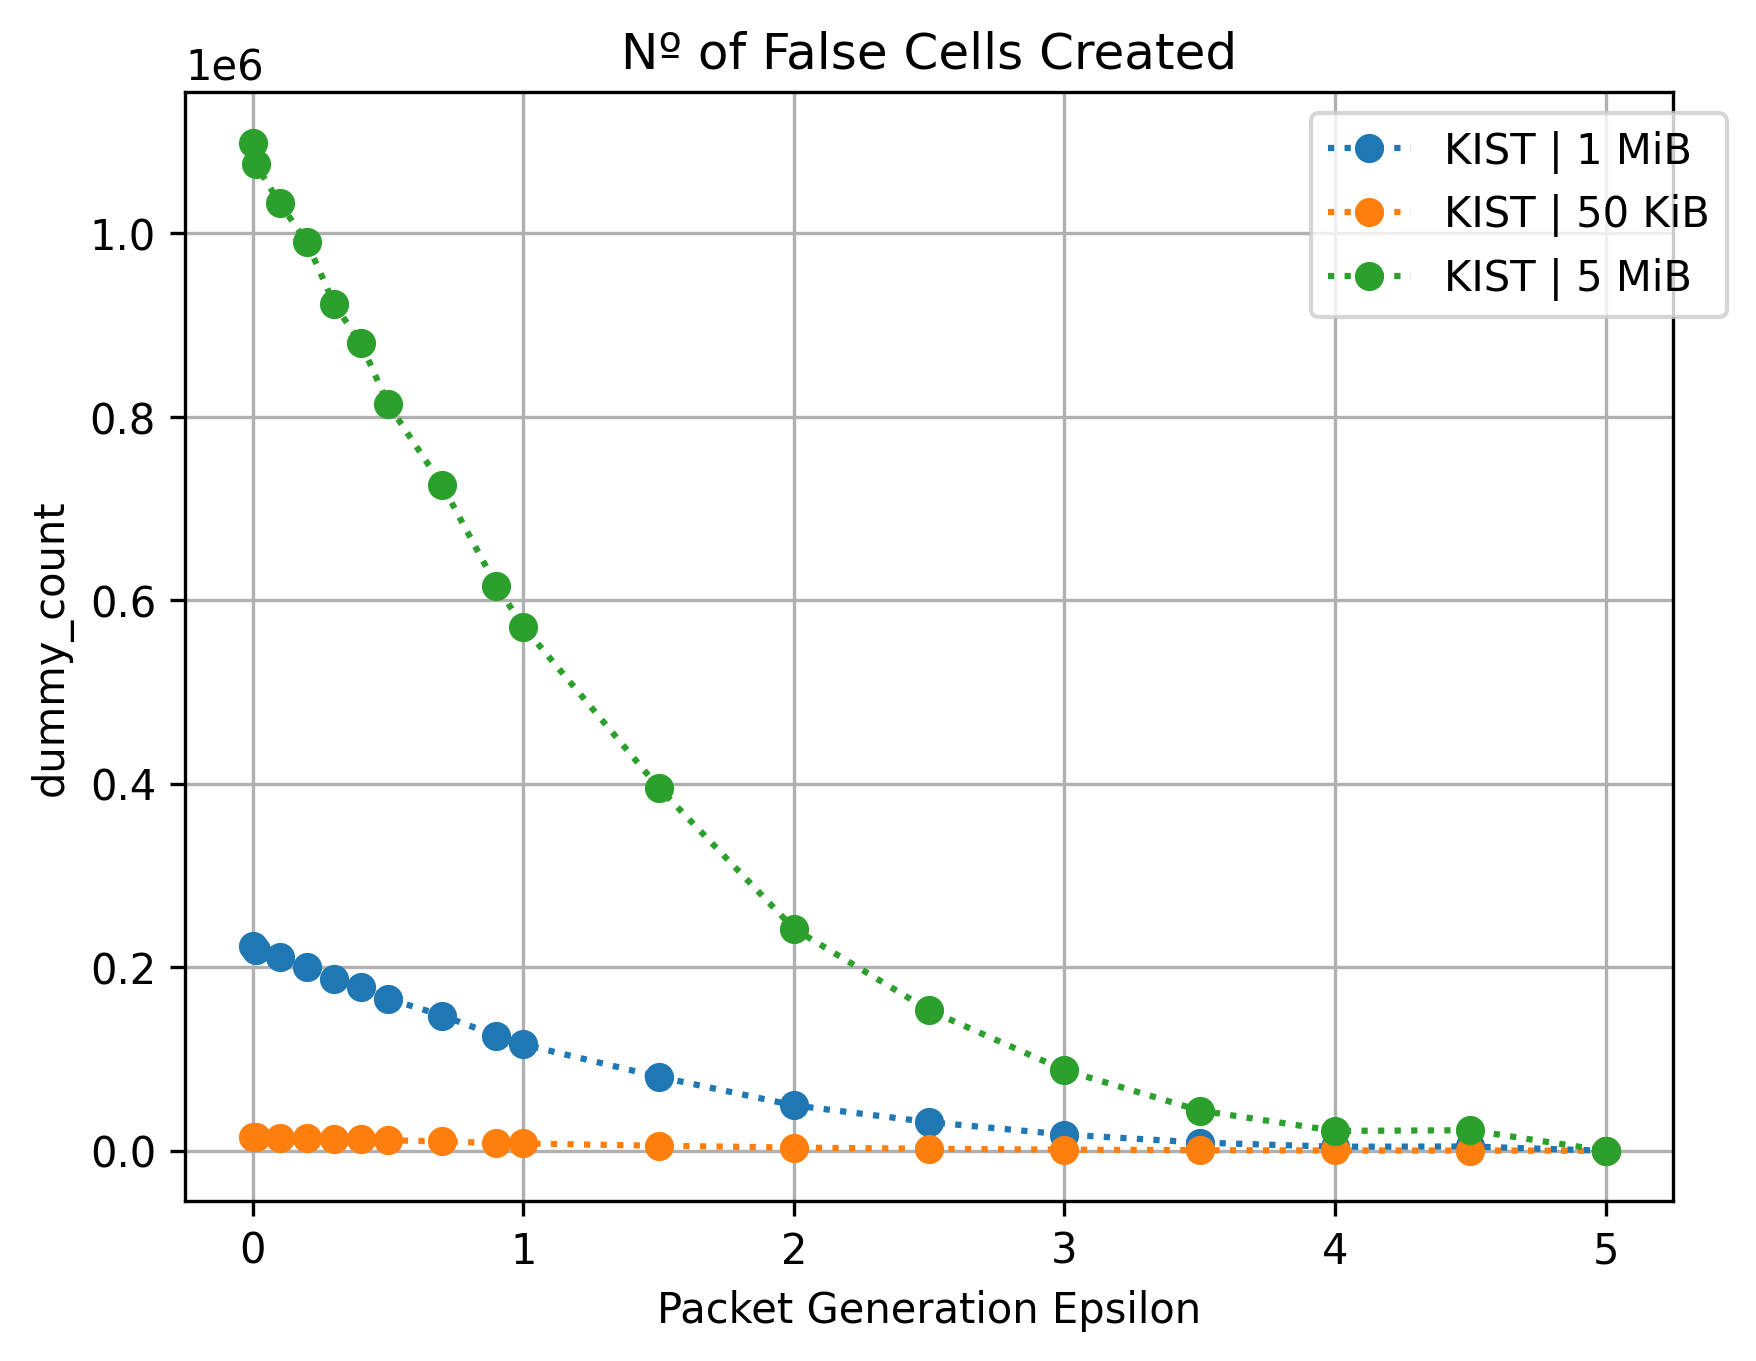
\includegraphics[width=\linewidth]{Chapters/Figures/Plots/Dummy/dummy_count_.png}}
    \end{subcaptionbox}
    \hfill
    \begin{subcaptionbox}{Packet Padding Cells Ratio\label{fig:dummy_ppc_ratio}}[0.3\textwidth]
        {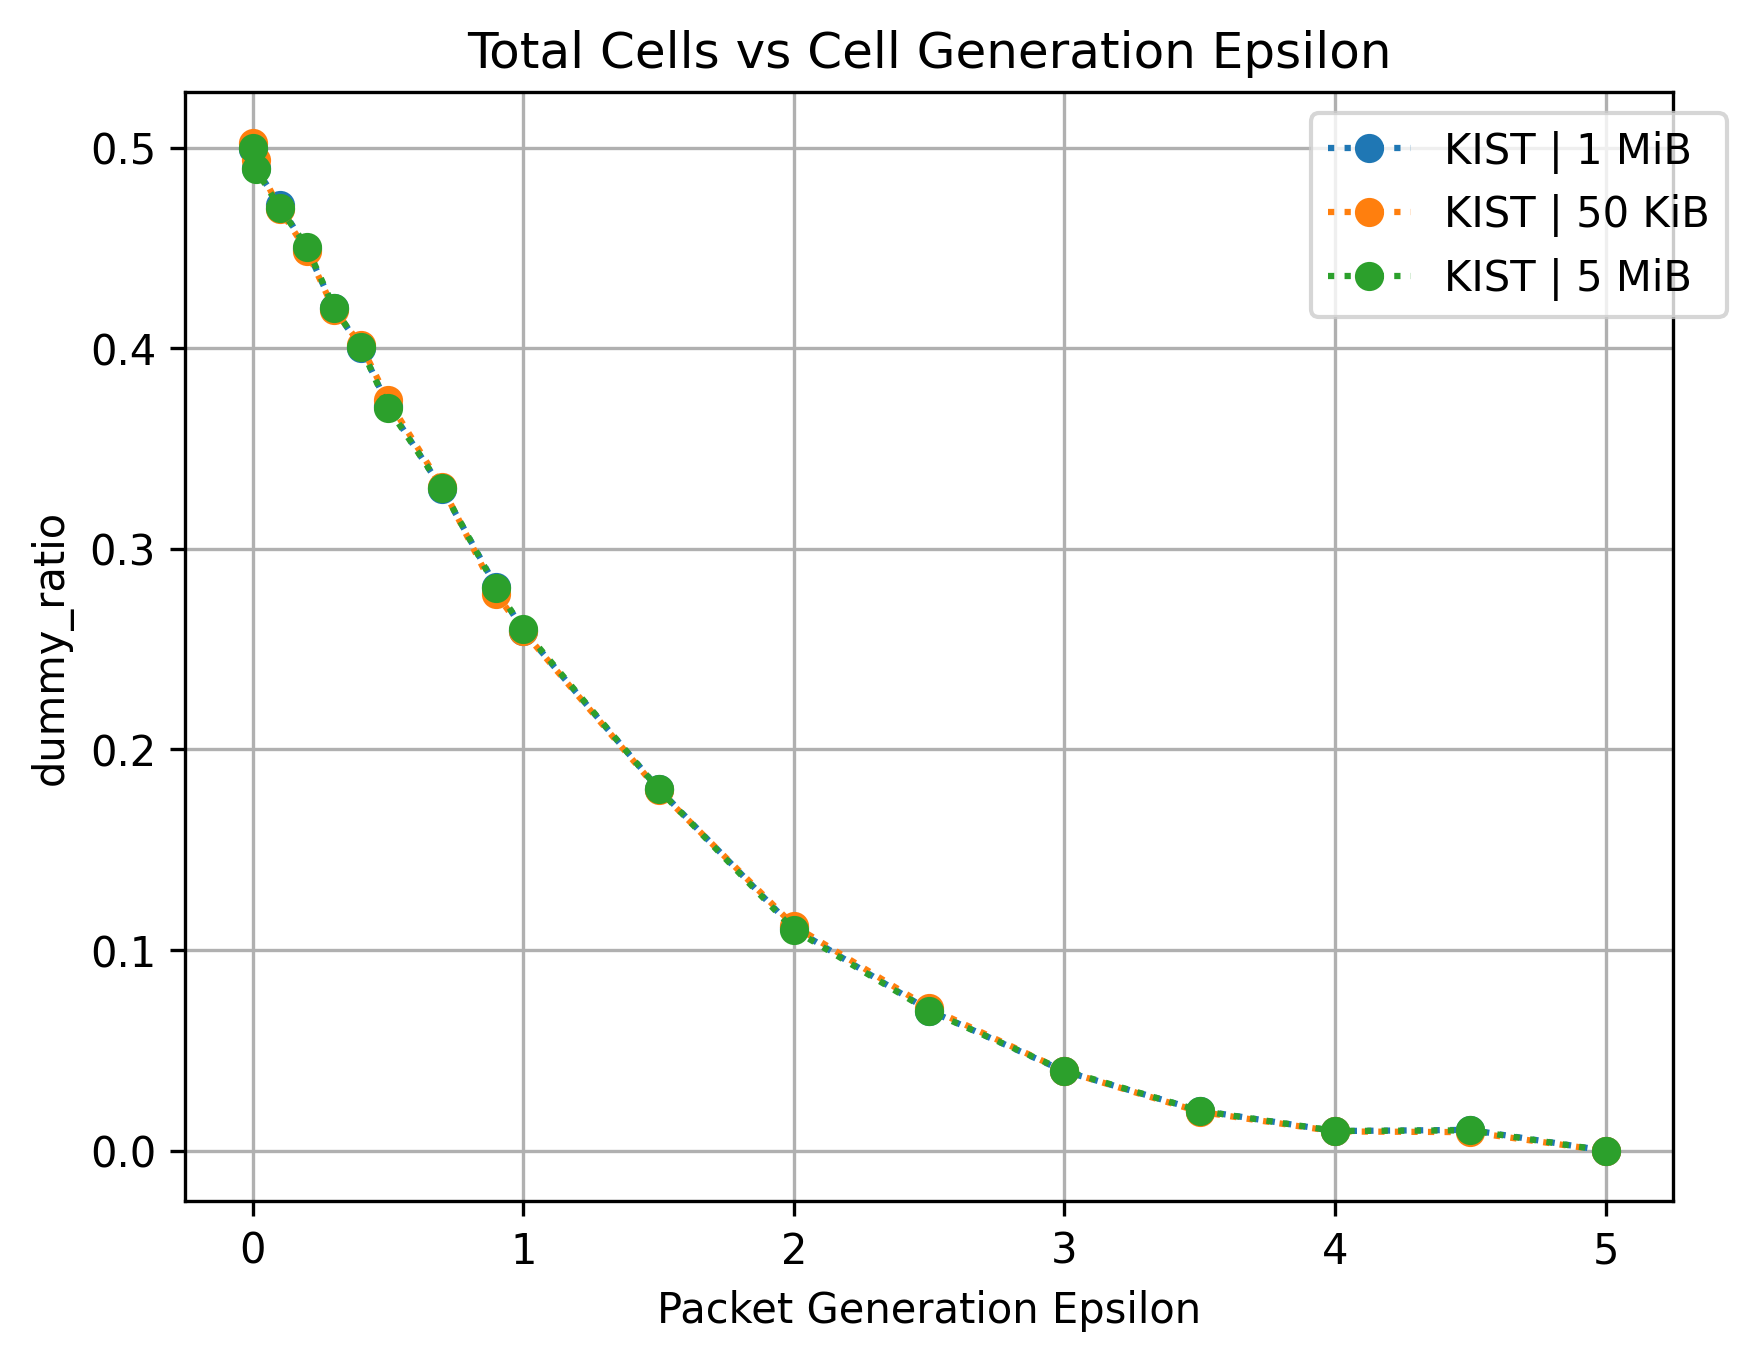
\includegraphics[width=\linewidth]{Chapters/Figures/Plots/Dummy/dummy_ratio_50_kib.png}}
    \end{subcaptionbox}
    \hfill
    \begin{subcaptionbox}{Total TLS Packets\label{fig:dummy_total_tls_packets}}[0.3\textwidth]
        {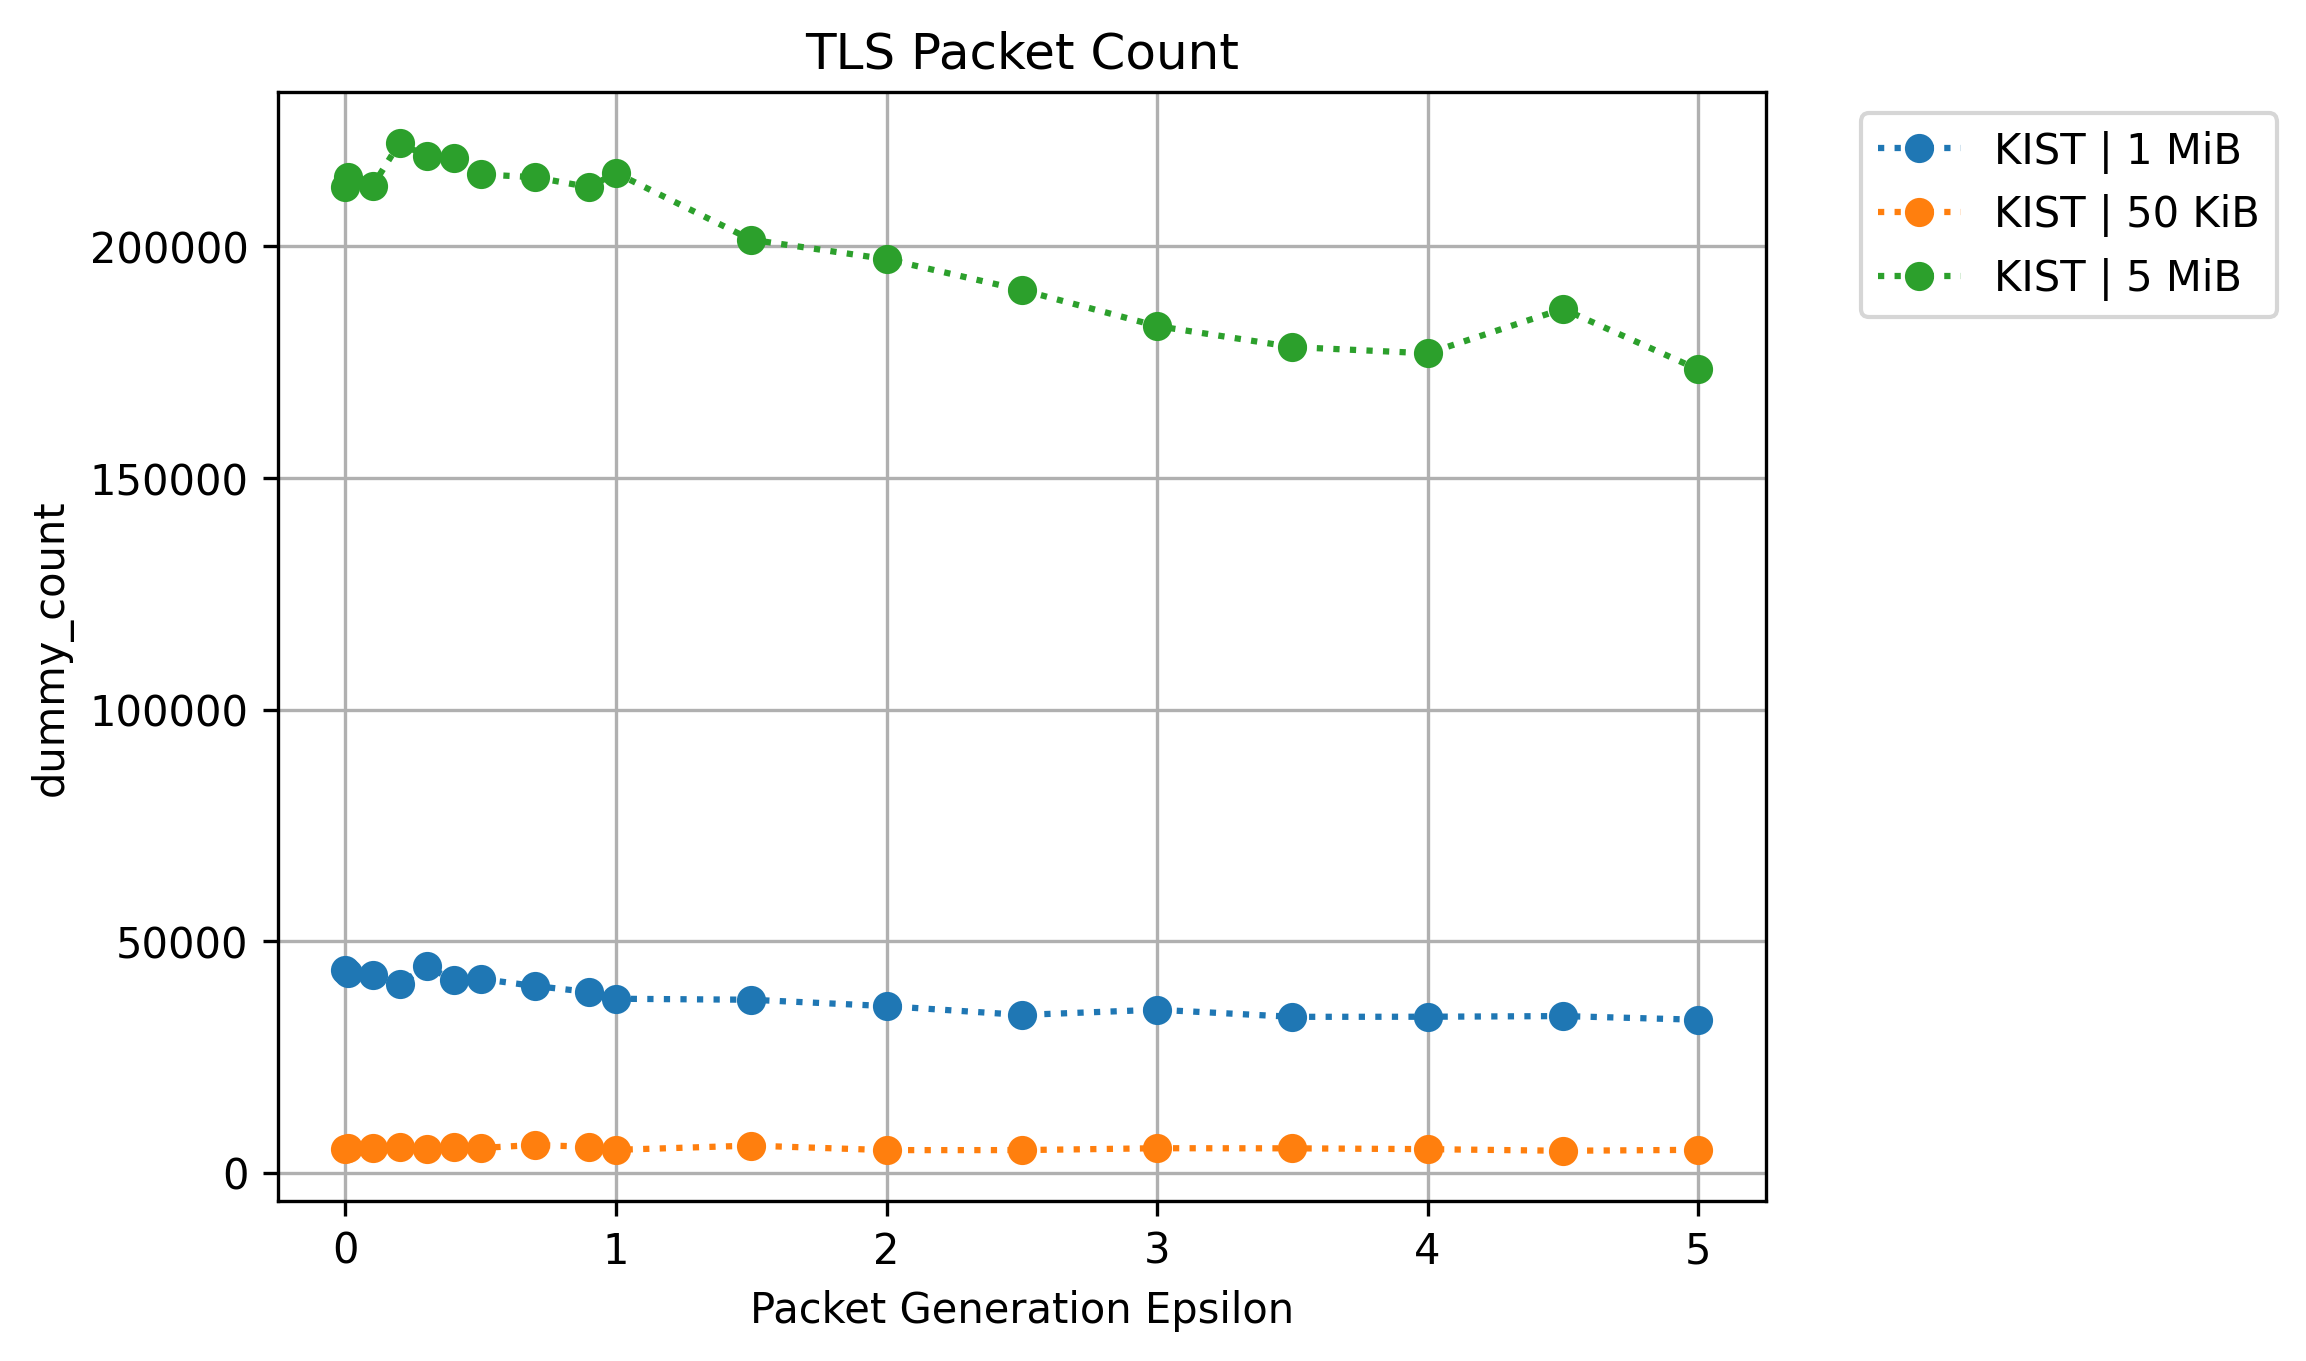
\includegraphics[width=\linewidth]{Chapters/Figures/Plots/Dummy/packet_count_50_kib.png}}
    \end{subcaptionbox}
    \caption{Packet Padding Cells Generation and Impact}\label{fig:dummy_ppc_analysis}
\end{figure}

Thee lower the $\epsilon$, more PPCs are generated and the higher the ratio of PPCs to total cells. However, it is important to note that the number of total TLS packets does not correspond to the cells graphic. This is because each TLS packet can contain multiple cells, and the number of cells is not directly proportional to the number of packets. 

\subsubsection{Latency}\label{sec:performance_evaluation_latency_tls_packets}

\begin{figure}[htbp]
    \centering
    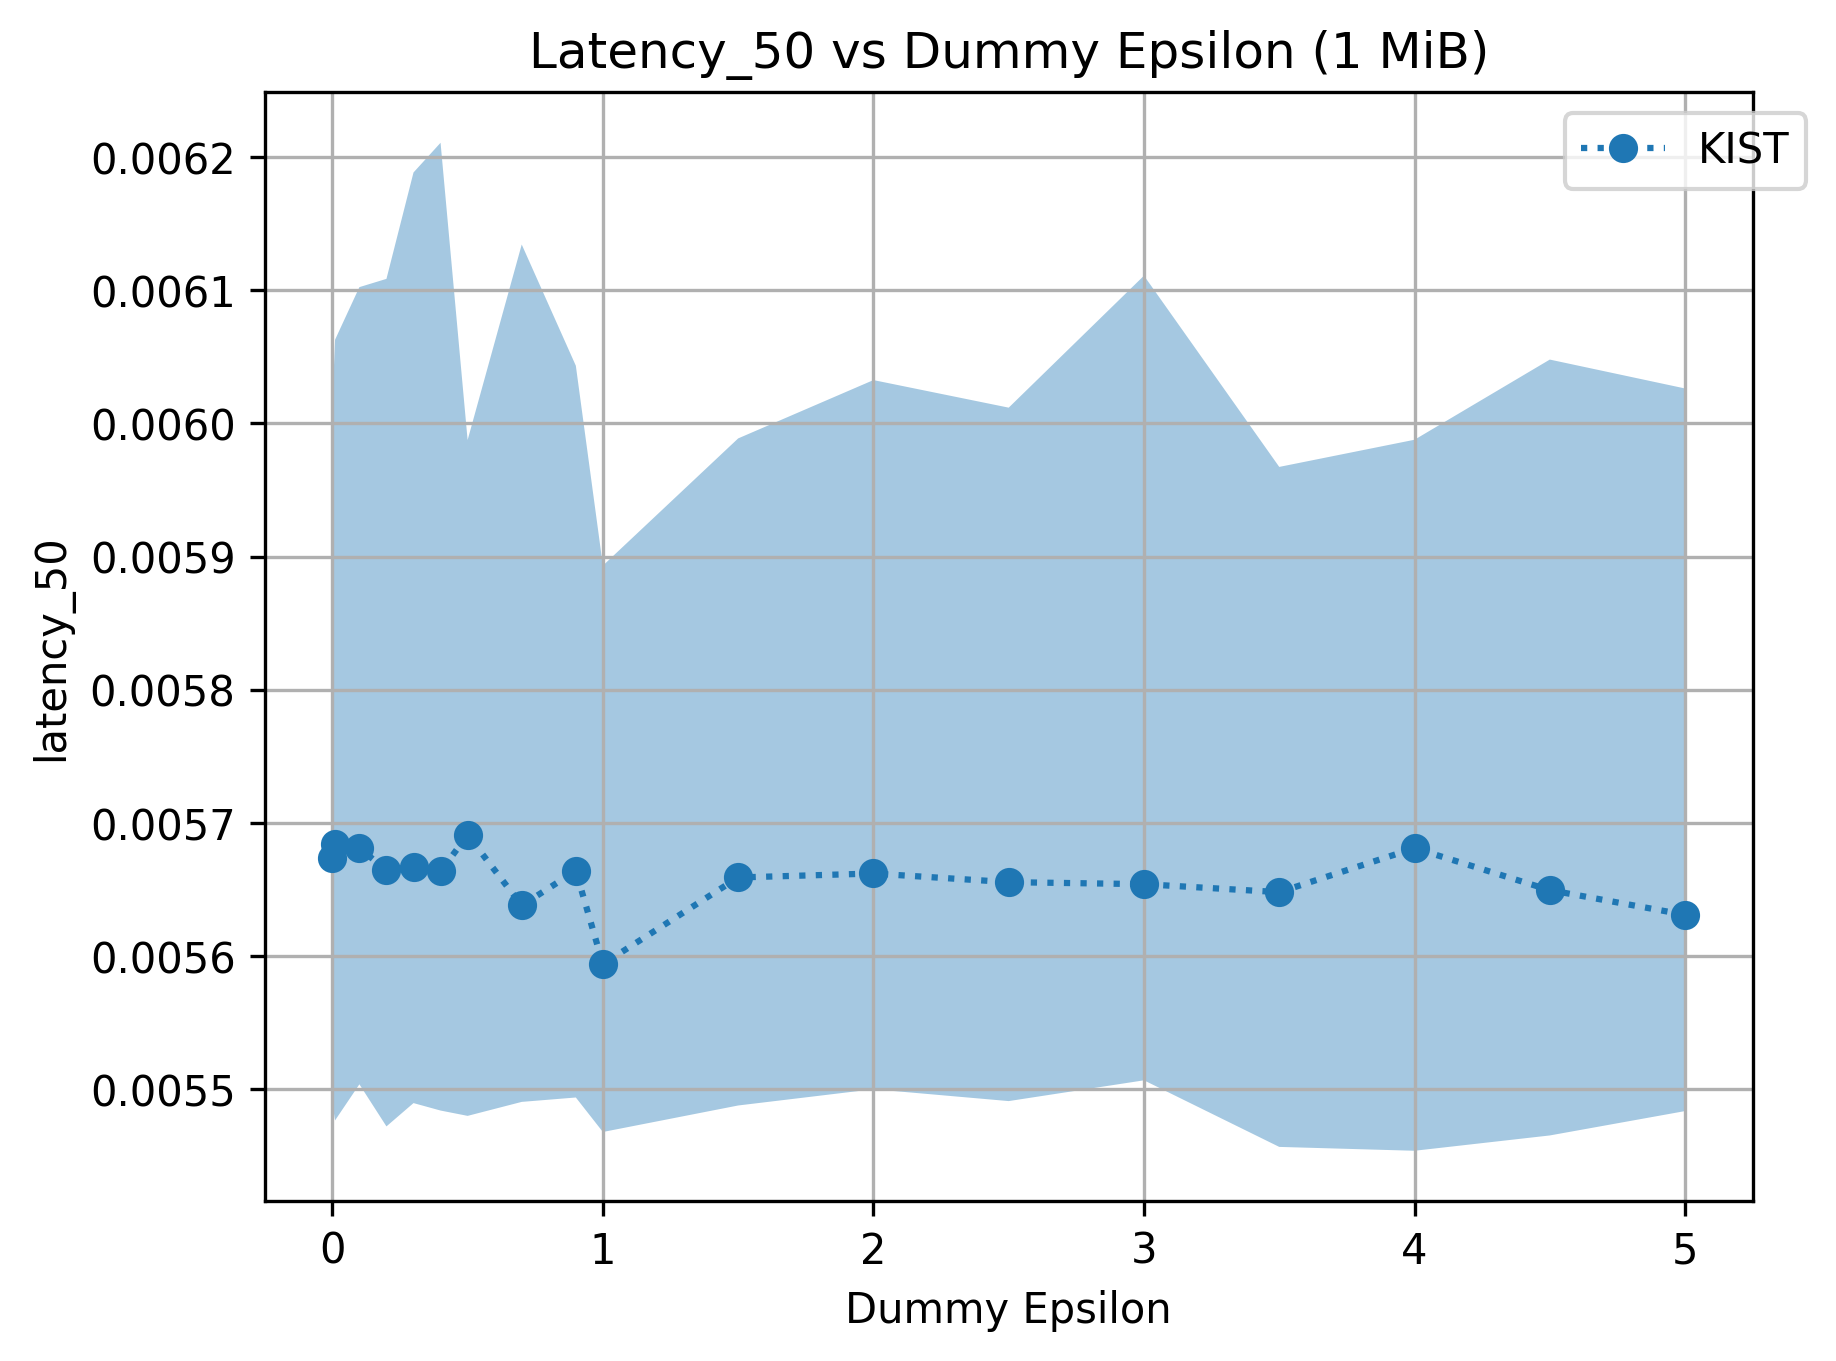
\includegraphics[scale=0.4]{Chapters/Figures/Plots/Dummy/latency_50_dummy_1_mib.png}
    \caption{Download Latency with Packet Padding Cells Generation}\label{fig:dummy_latency_tls_packets}
\end{figure}

The latency keeps in the same range across all tested $\epsilon$ with higher percentile 90 values near lower values. The median latency of all tests concentrates between 0.0056 and 0.0057 seconds.

\subsubsection{Throughput}\label{sec:performance_evaluation_throughput_tls_packets}

\begin{figure}[htbp]
    \centering
    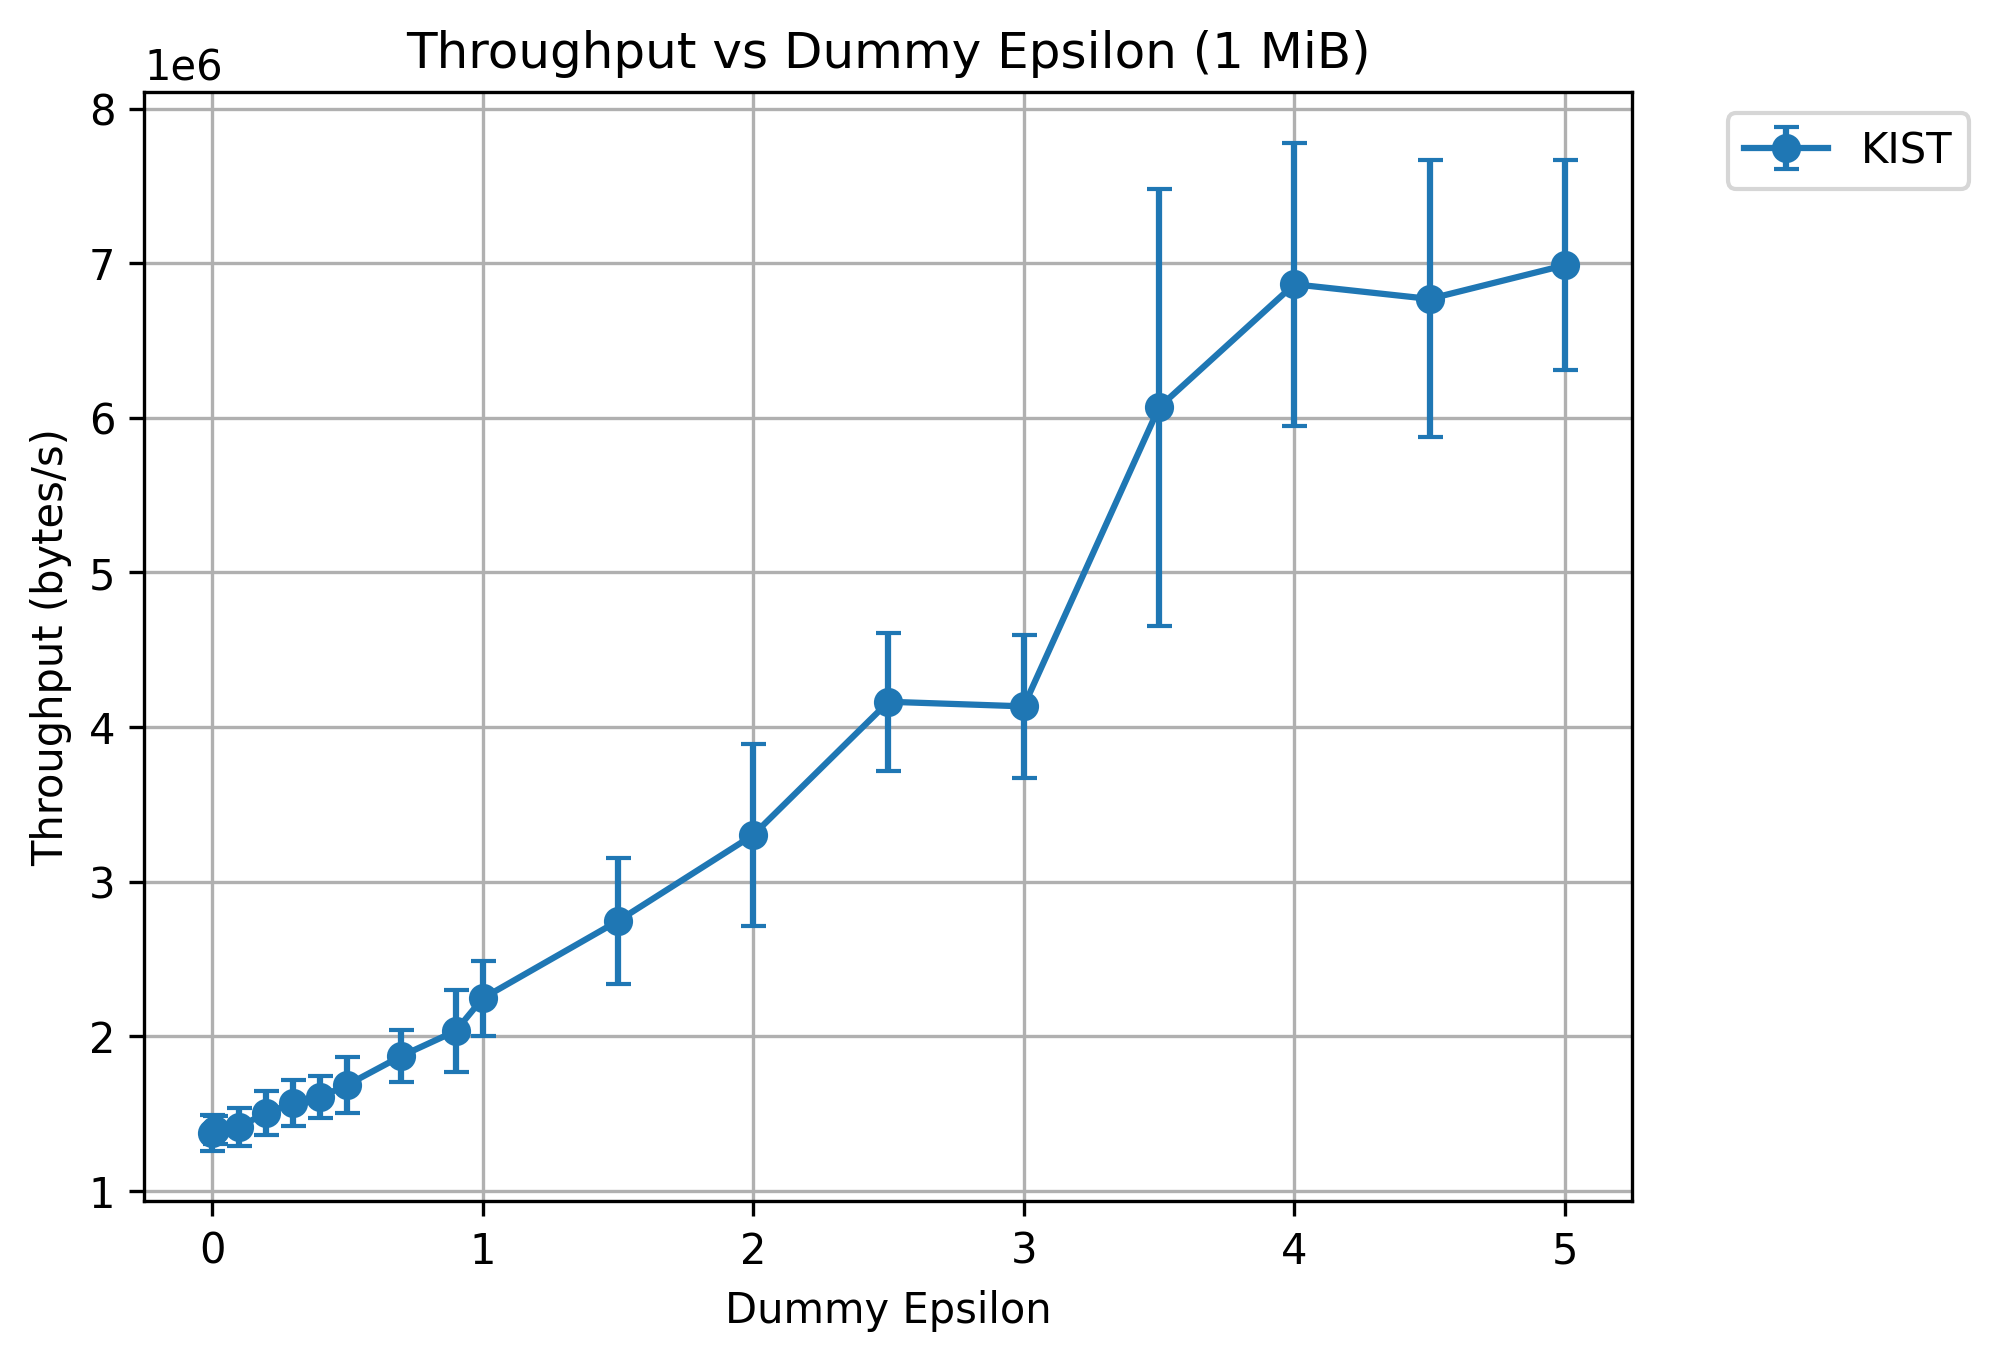
\includegraphics[scale=0.4]{Chapters/Figures/Plots/Dummy/throughput_dummy_1_mib.png}
    \caption{Download Throughput with Packet Padding Cells Generation}\label{fig:dummy_throughput_tls_packets}
\end{figure}

The throughput gets higher as the $\epsilon$ increases, as expected, and the standard deviation also increases.

\subsubsection{Total Time}

\begin{figure}[htbp]
    \centering
    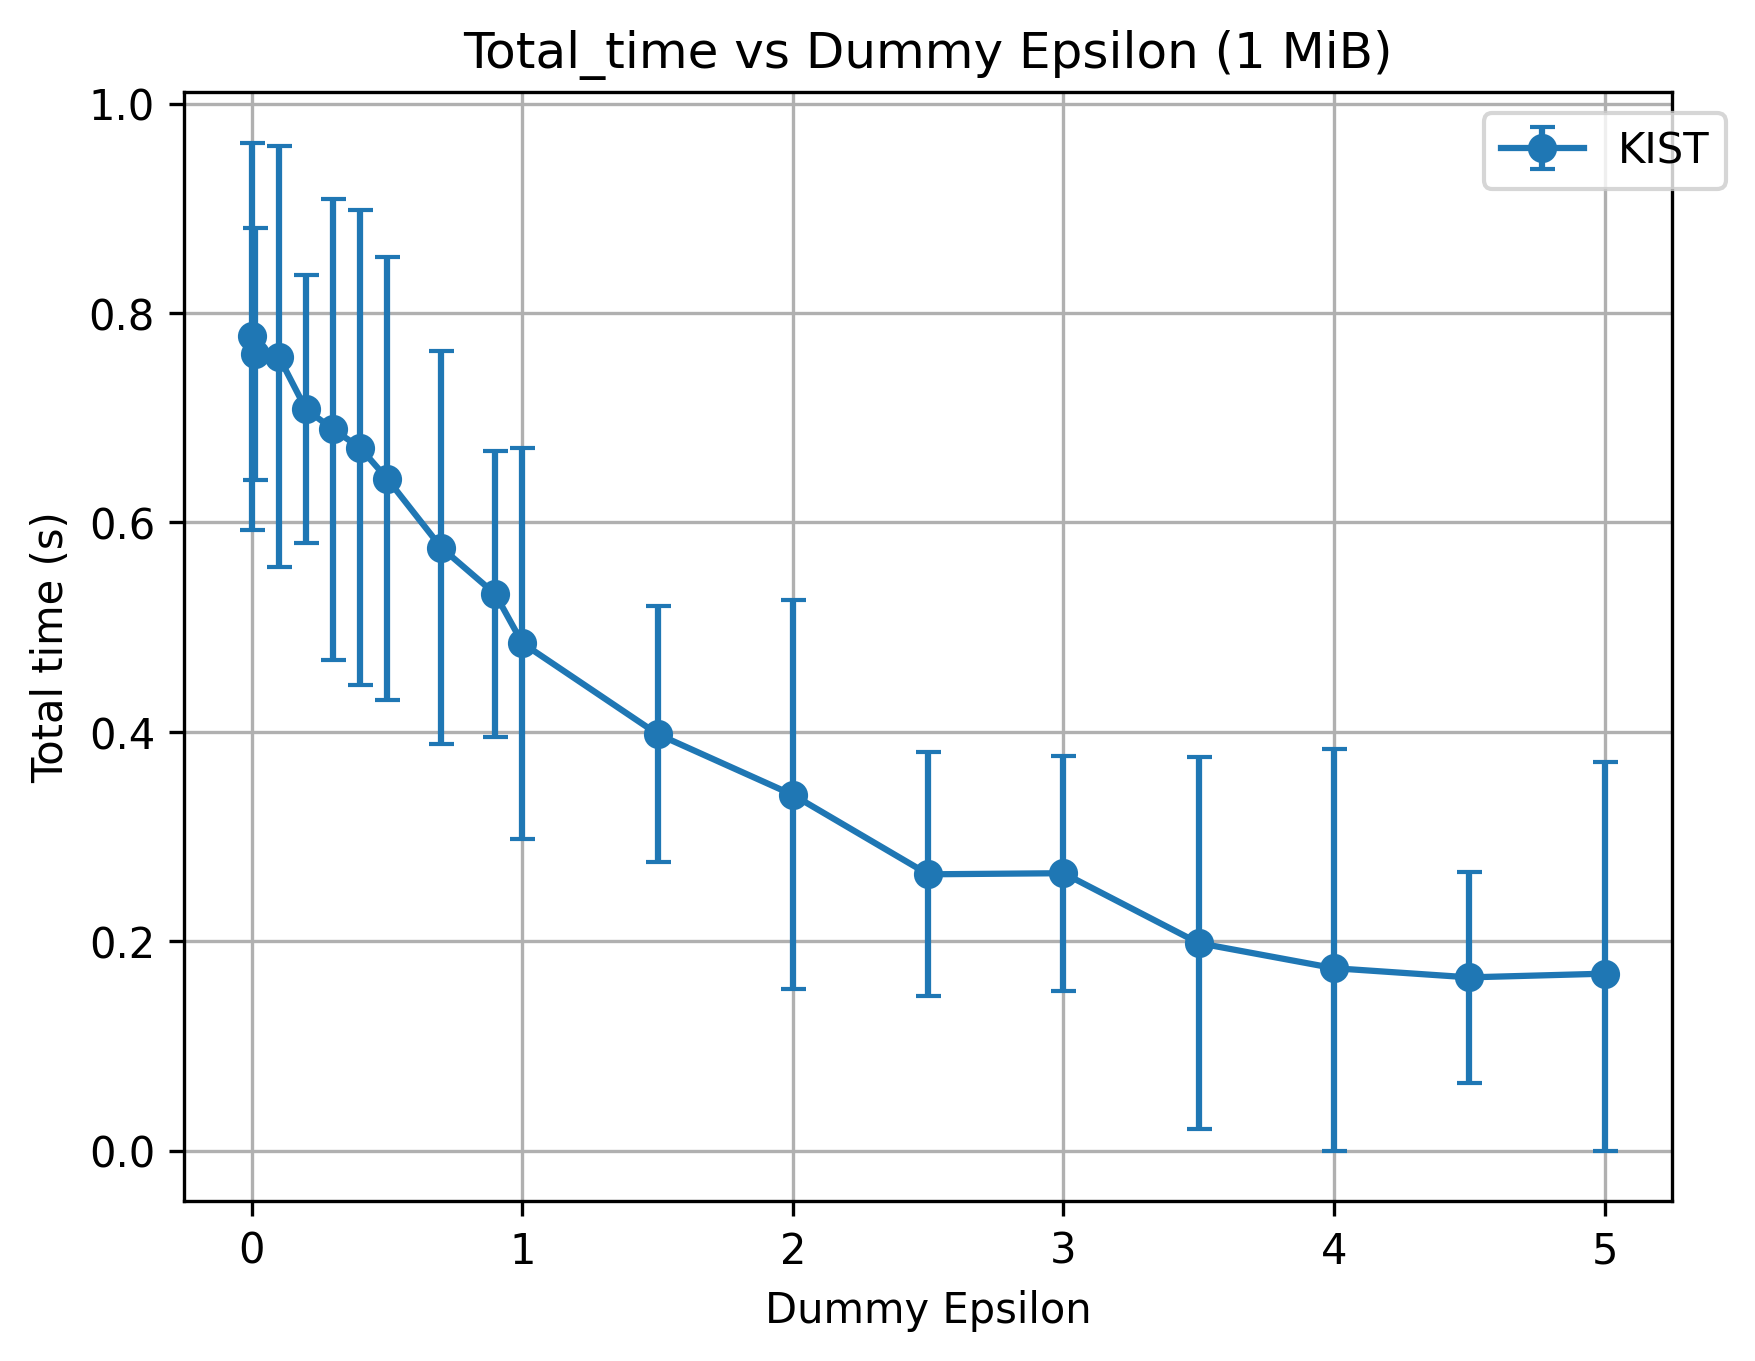
\includegraphics[scale=0.4]{Chapters/Figures/Plots/Dummy/total_time_dummy_1_mib.png}
    \caption{Download Total Time with Packet Padding Cells Generation}\label{fig:dummy_total_time_tls_packets}
\end{figure}

The total time needed to download the file decreases as the $\epsilon$ gets higher, as expected. The standard deviation keeps similar values across all tests.

\subsection{Jitter Injector Tor Schedulers}\label{sec:performance_evaluation_jitter_injectors_tor_schedulers}

To evaluate the performance of the new implemented Priv\_KIST and Priv\_Vanilla Tor Schedulers, we downloaded a file from a web server using curl. The tests were performed 100 times, with different schedulers, with variable $\epsilon$ values, ranging from 0 to 10 and using 1 of the following mathematical distributions to generate jitter: Laplace, Poisson and Exponential. The file size was set to 1 MiB.

\subsubsection{Latency}\label{sec:performance_evaluation_latency_jitter_injectors_tor_schedulers}

\begin{figure}[htbp]
    \centering
    \begin{subcaptionbox}{Laplace Distribution\label{fig:jitter_latency_laplace}}[0.45\textwidth]
        {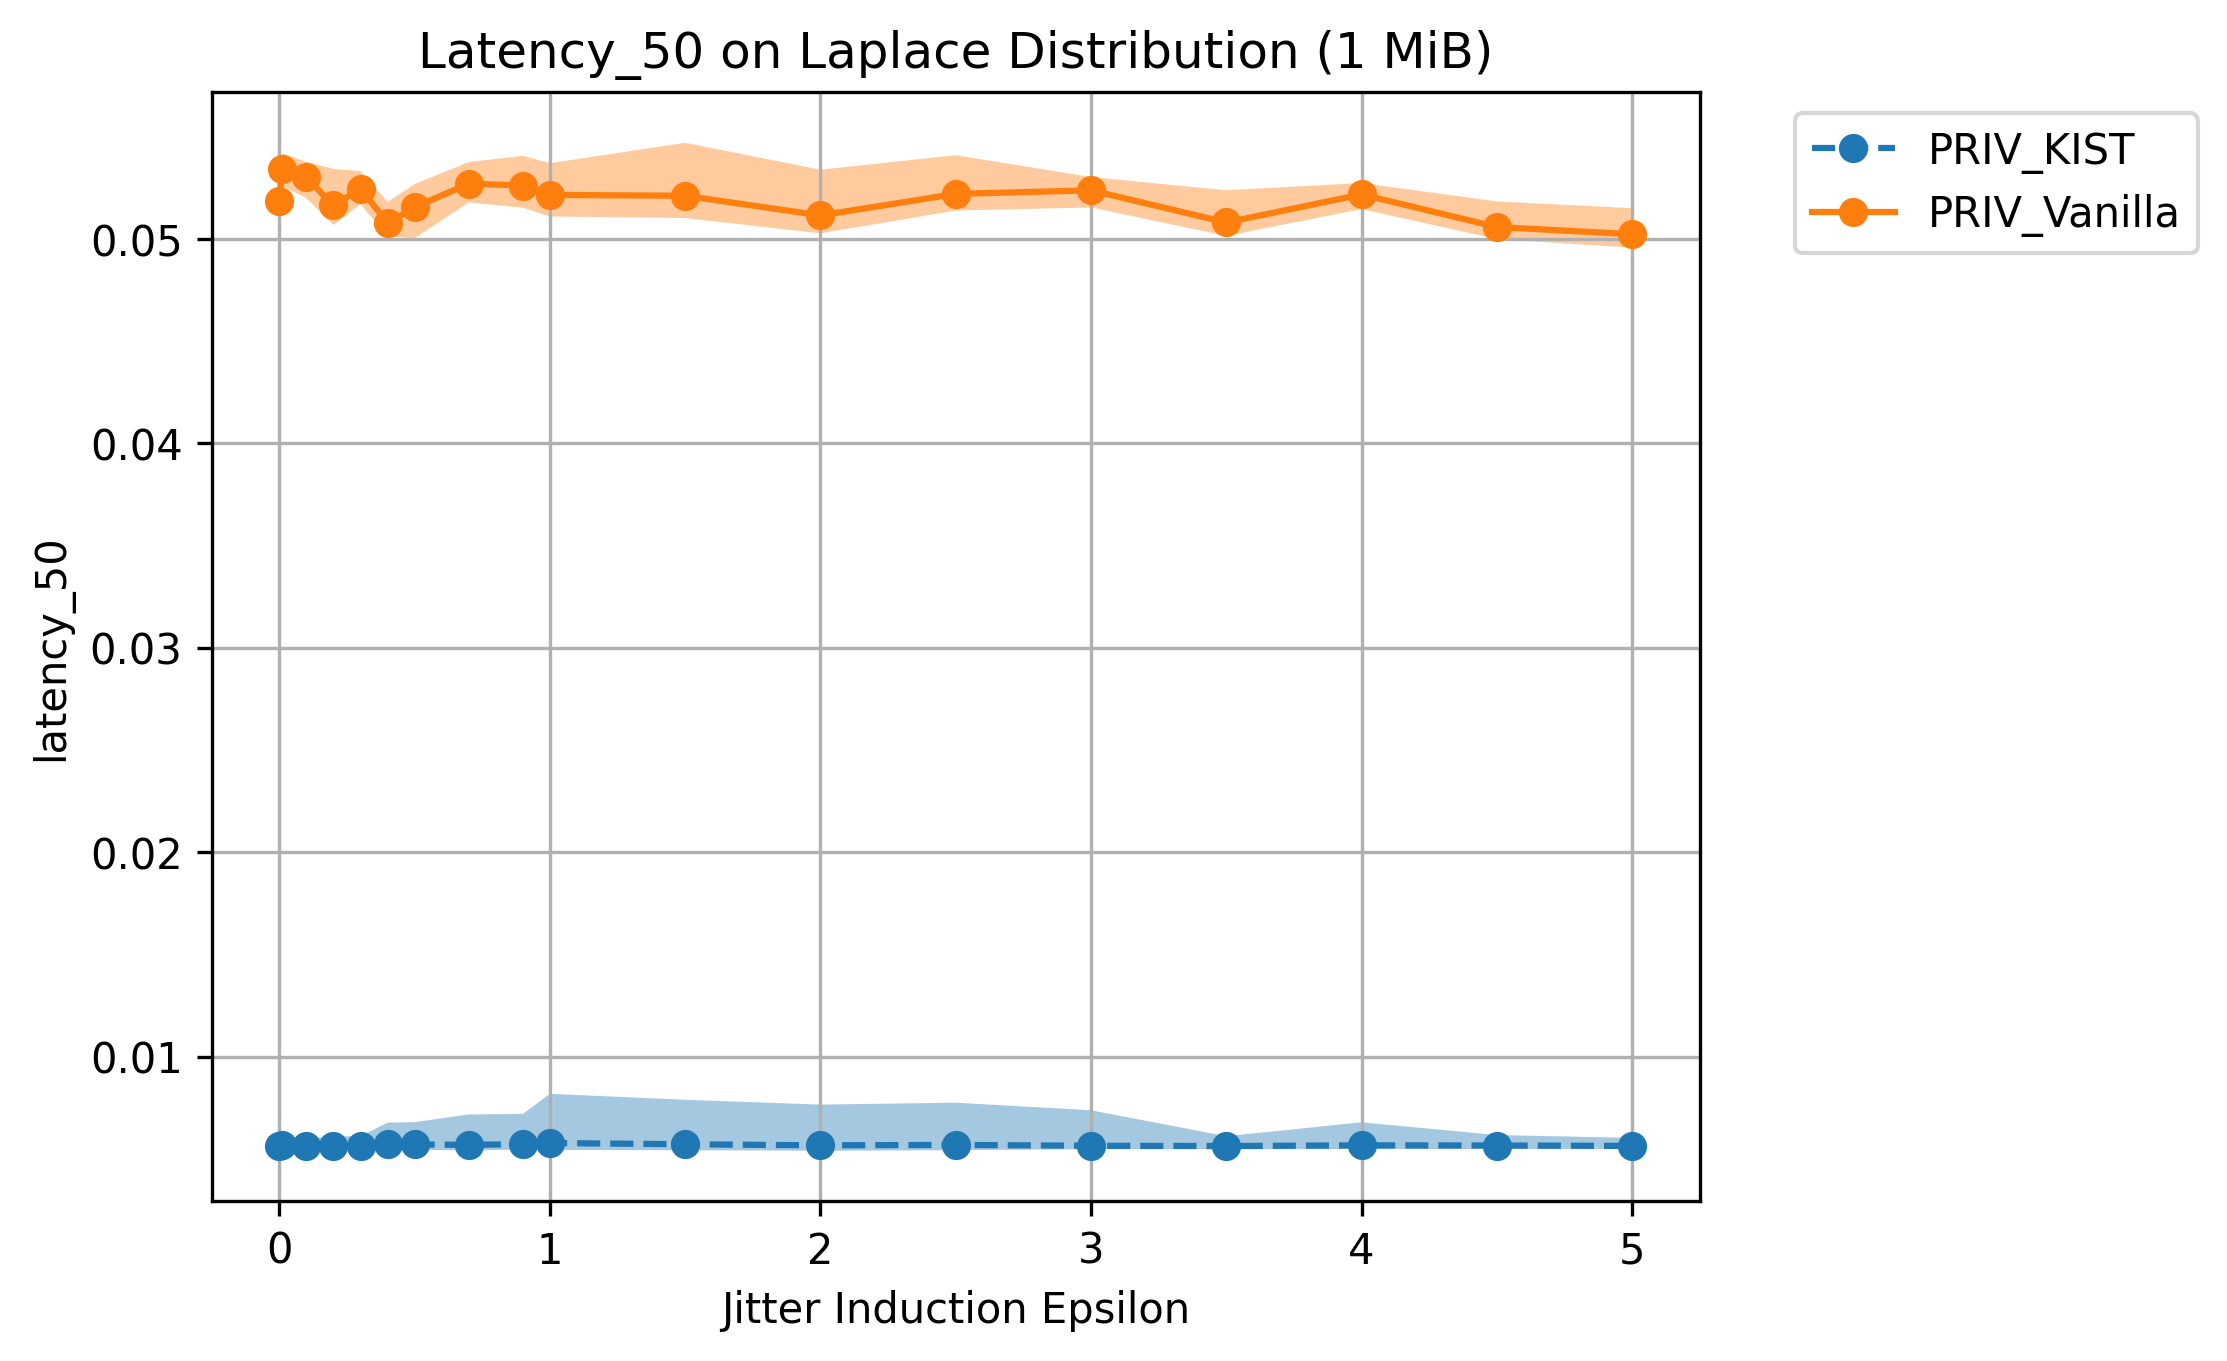
\includegraphics[width=\linewidth]{Chapters/Figures/Plots/Jitter/latency_jitter_Laplace_1_mib.png}}
    \end{subcaptionbox}
    \hfill
    \begin{subcaptionbox}{Exponential Distribution\label{fig:jitter_latency_exponential}}[0.45\textwidth]
        {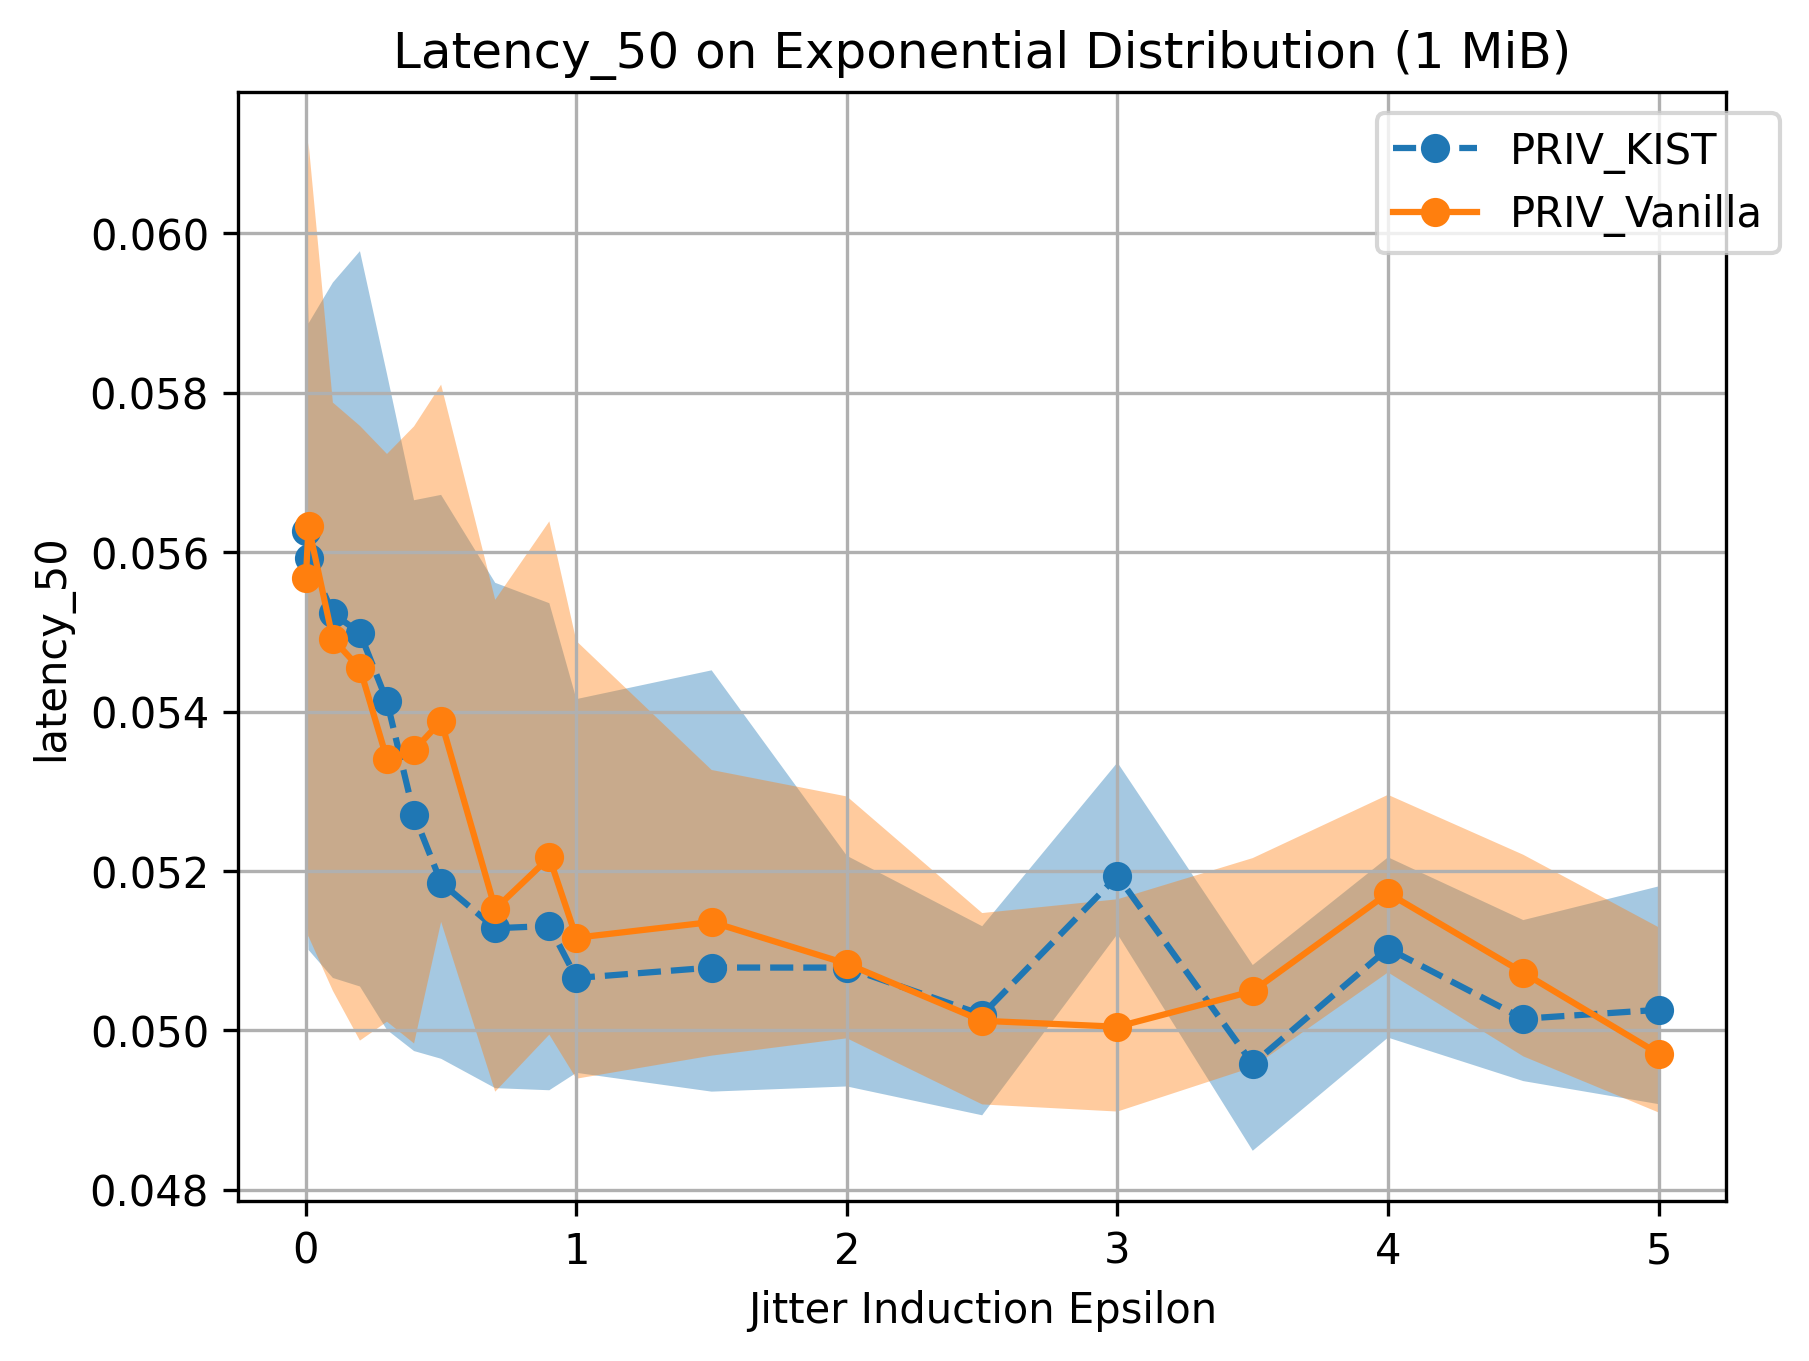
\includegraphics[width=\linewidth]{Chapters/Figures/Plots/Jitter/latency_jitter_Exponential_1_mib.png}}
    \end{subcaptionbox}
    \hfill
    \begin{subcaptionbox}{Poisson Distribution\label{fig:jitter_latency_poisson}}[0.45\textwidth]
        {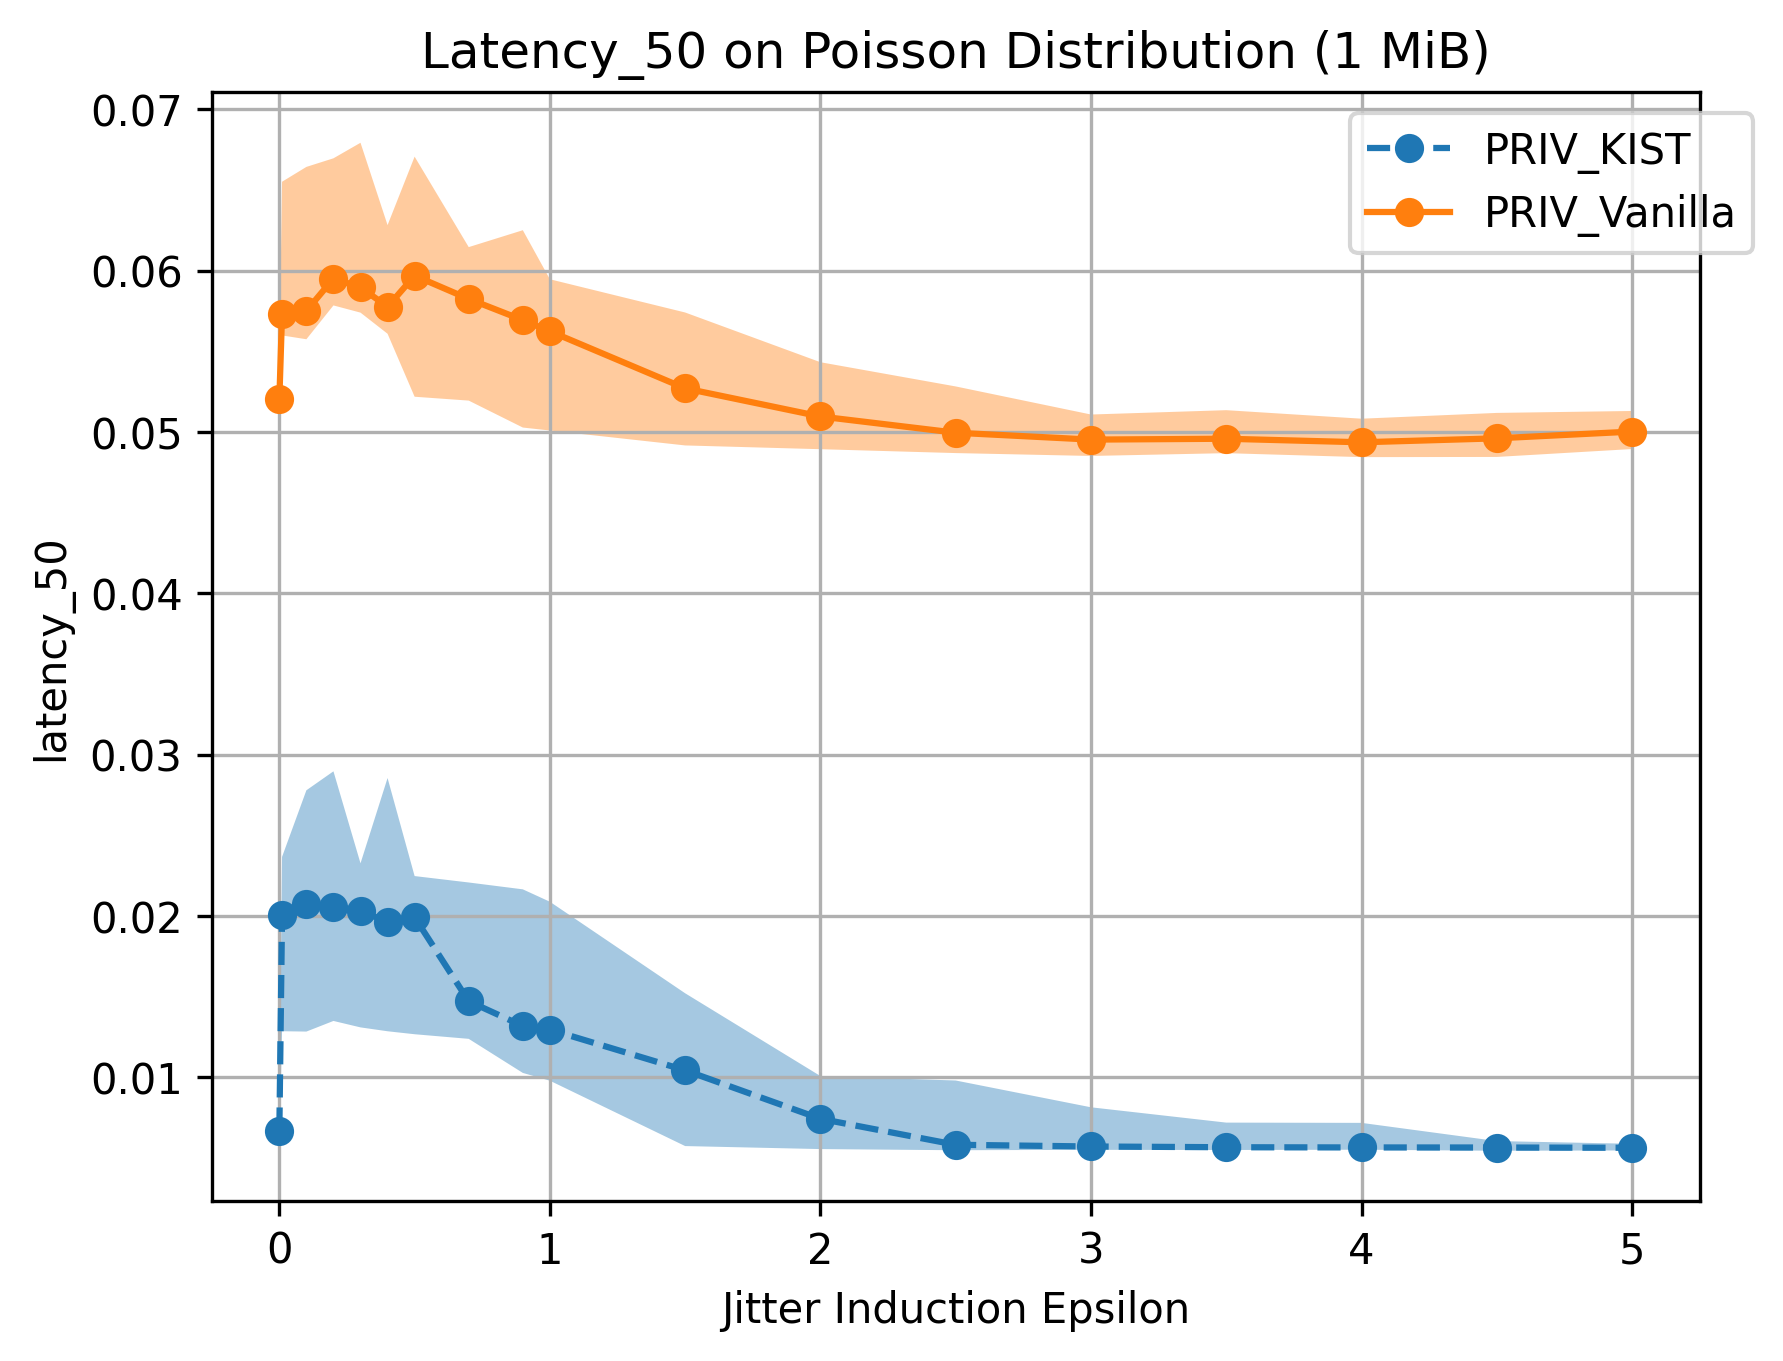
\includegraphics[width=\linewidth]{Chapters/Figures/Plots/Jitter/latency_jitter_Poisson_1_mib.png}}
    \end{subcaptionbox}
    \hfill
    \begin{subcaptionbox}{All Distributions\label{fig:jitter_latency_all}}[0.45\textwidth]
        {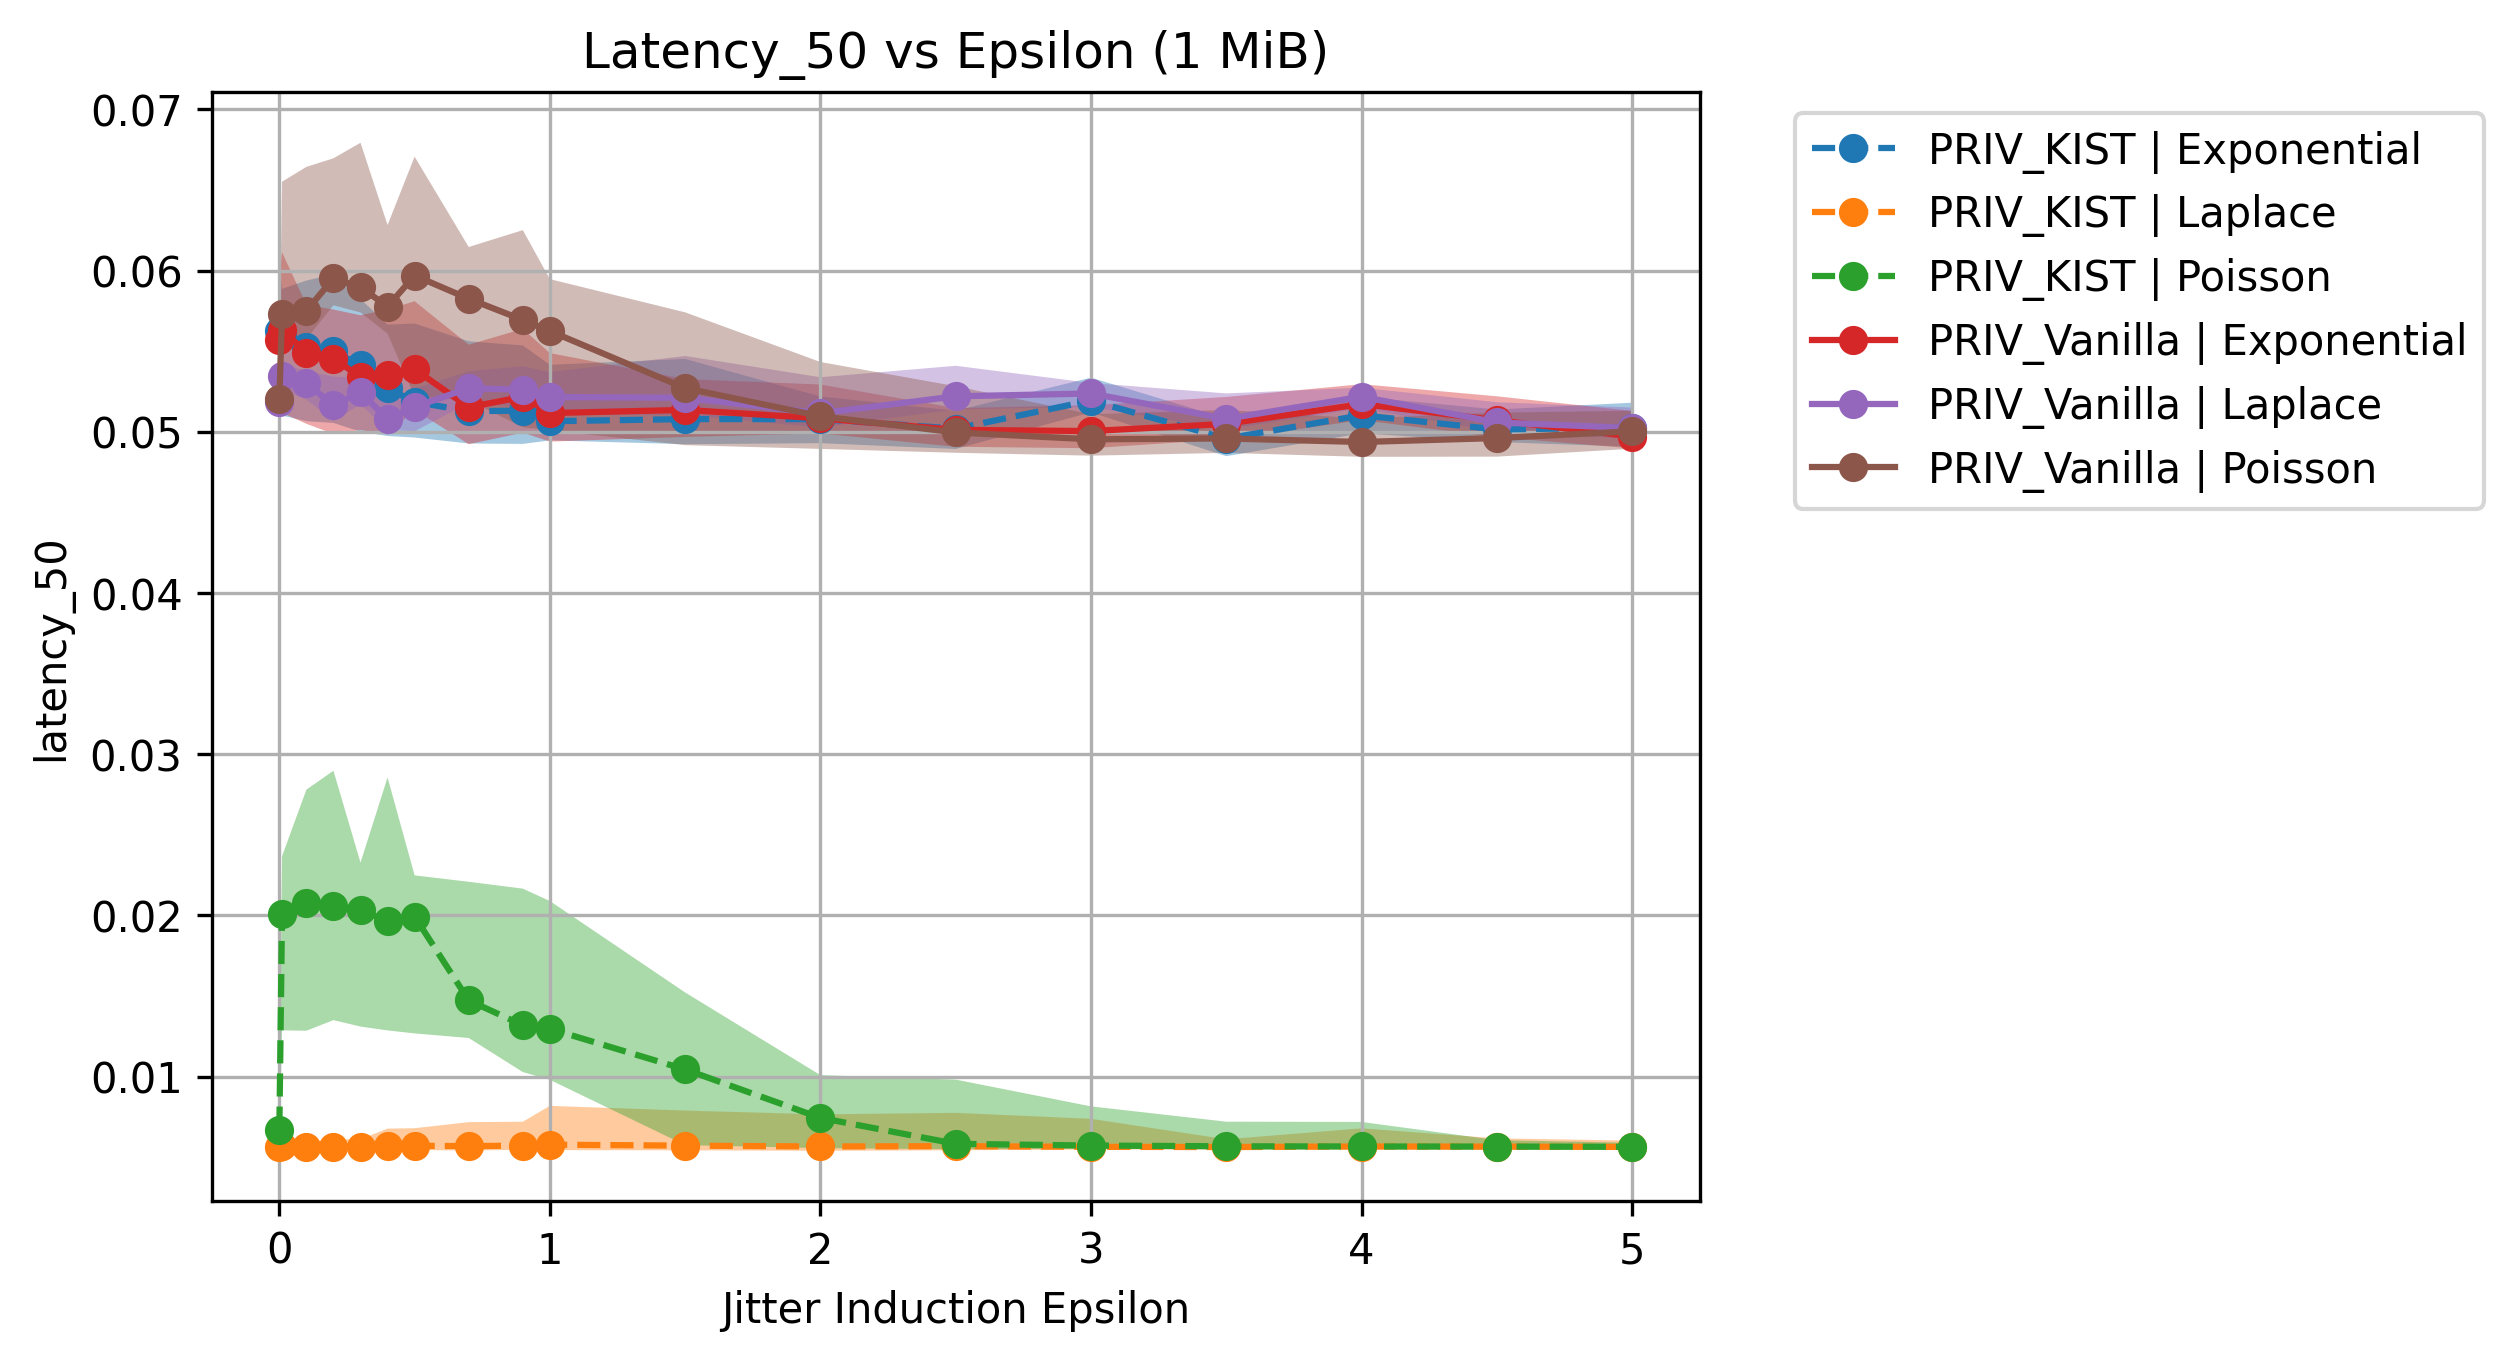
\includegraphics[width=\linewidth]{Chapters/Figures/Plots/Jitter/latency_jitter_1_mib.png}}
    \end{subcaptionbox}
    \caption{Tor Schedulers and Jitter Impact on Latency}\label{fig:jitter_latency_analysis}
\end{figure}

The Laplace Distribution tests show that latency is not affected by the injected jitter, as the median latency remains constant across all tests. 
The Poisson Distribution gets higher median latency values as the $\epsilon$ comes closer to 0 which then decreases and remains constant for $\epsilon$ values higher than 2,5.
The Exponential Distribution shows a similar behavior to the Poisson Distribution, but shows a more pronounced increase in median latency as the $\epsilon$ approaches 0, and a more variable behavior throughout the tests.

In comparison, regarding latency, the Laplace Distribution is the most stable, while the Poisson and Exponential Distributions show more variability in the results. The PRIV\_KIST scheduler performs better, with lower median latency values than the PRIV\_Vanilla scheduler, even thought the Exponential Distribution shows similar median latency values for both schedulers. 

\subsubsection{Throughput}\label{sec:performance_evaluation_throughput_jitter_injectors_tor_schedulers}

\begin{figure}[htbp]
    \centering
    \begin{subcaptionbox}{Laplace Distribution\label{fig:jitter_throughput_laplace}}[0.45\textwidth]
        {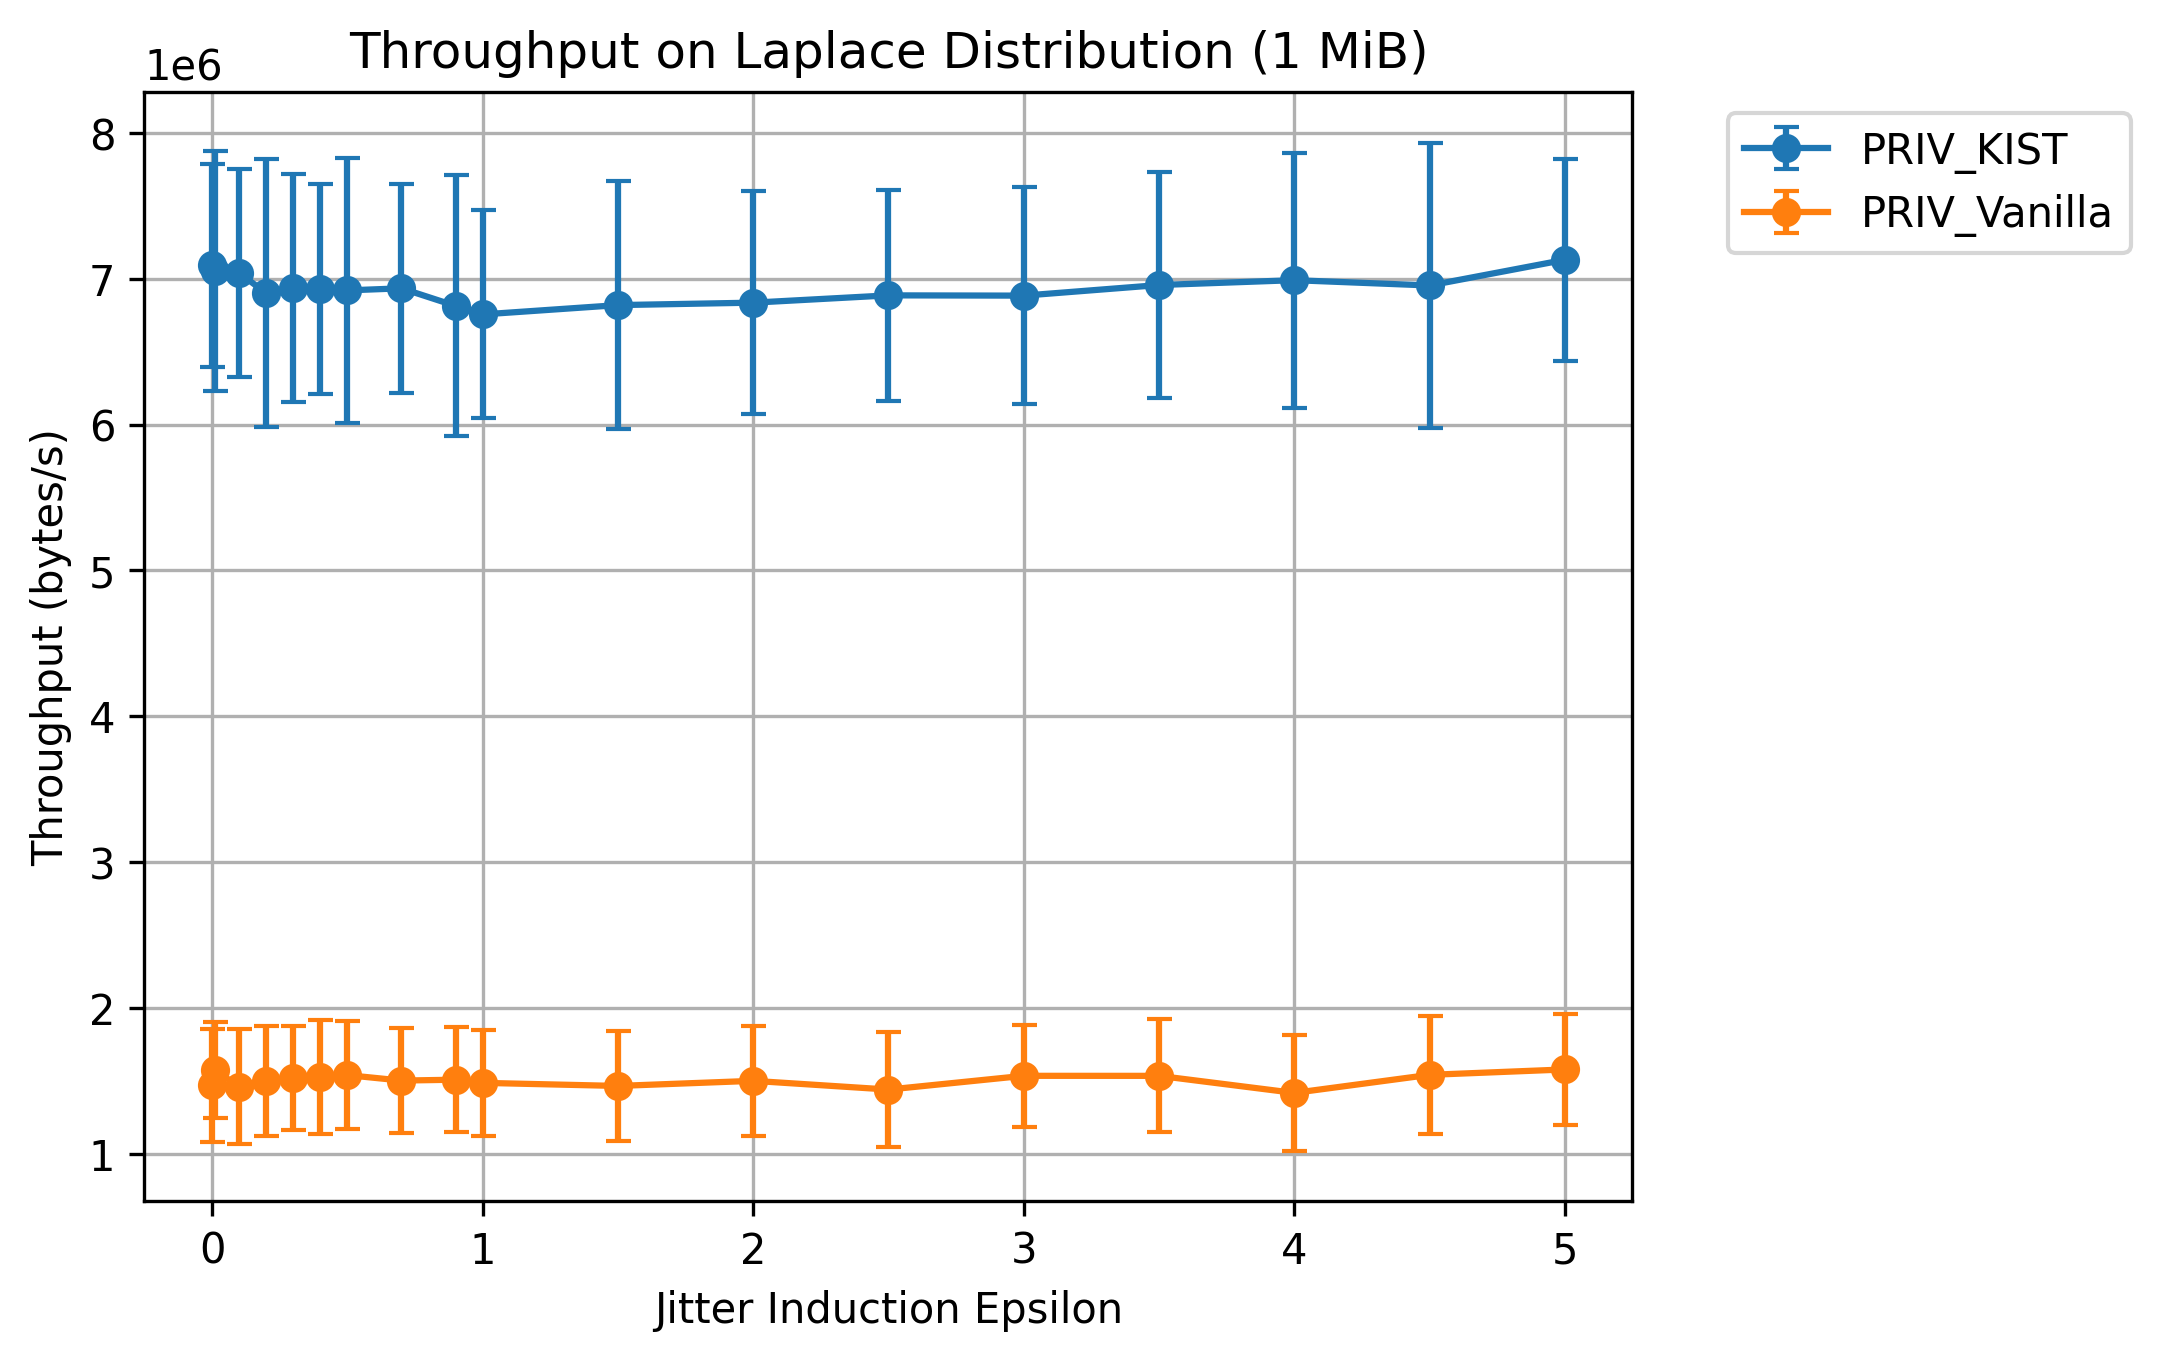
\includegraphics[width=\linewidth]{Chapters/Figures/Plots/Jitter/throughput_jitter_Laplace_1_mib.png}}
    \end{subcaptionbox}
    \hfill
    \begin{subcaptionbox}{Exponential Distribution\label{fig:jitter_throughput_exponential}}[0.45\textwidth]
        {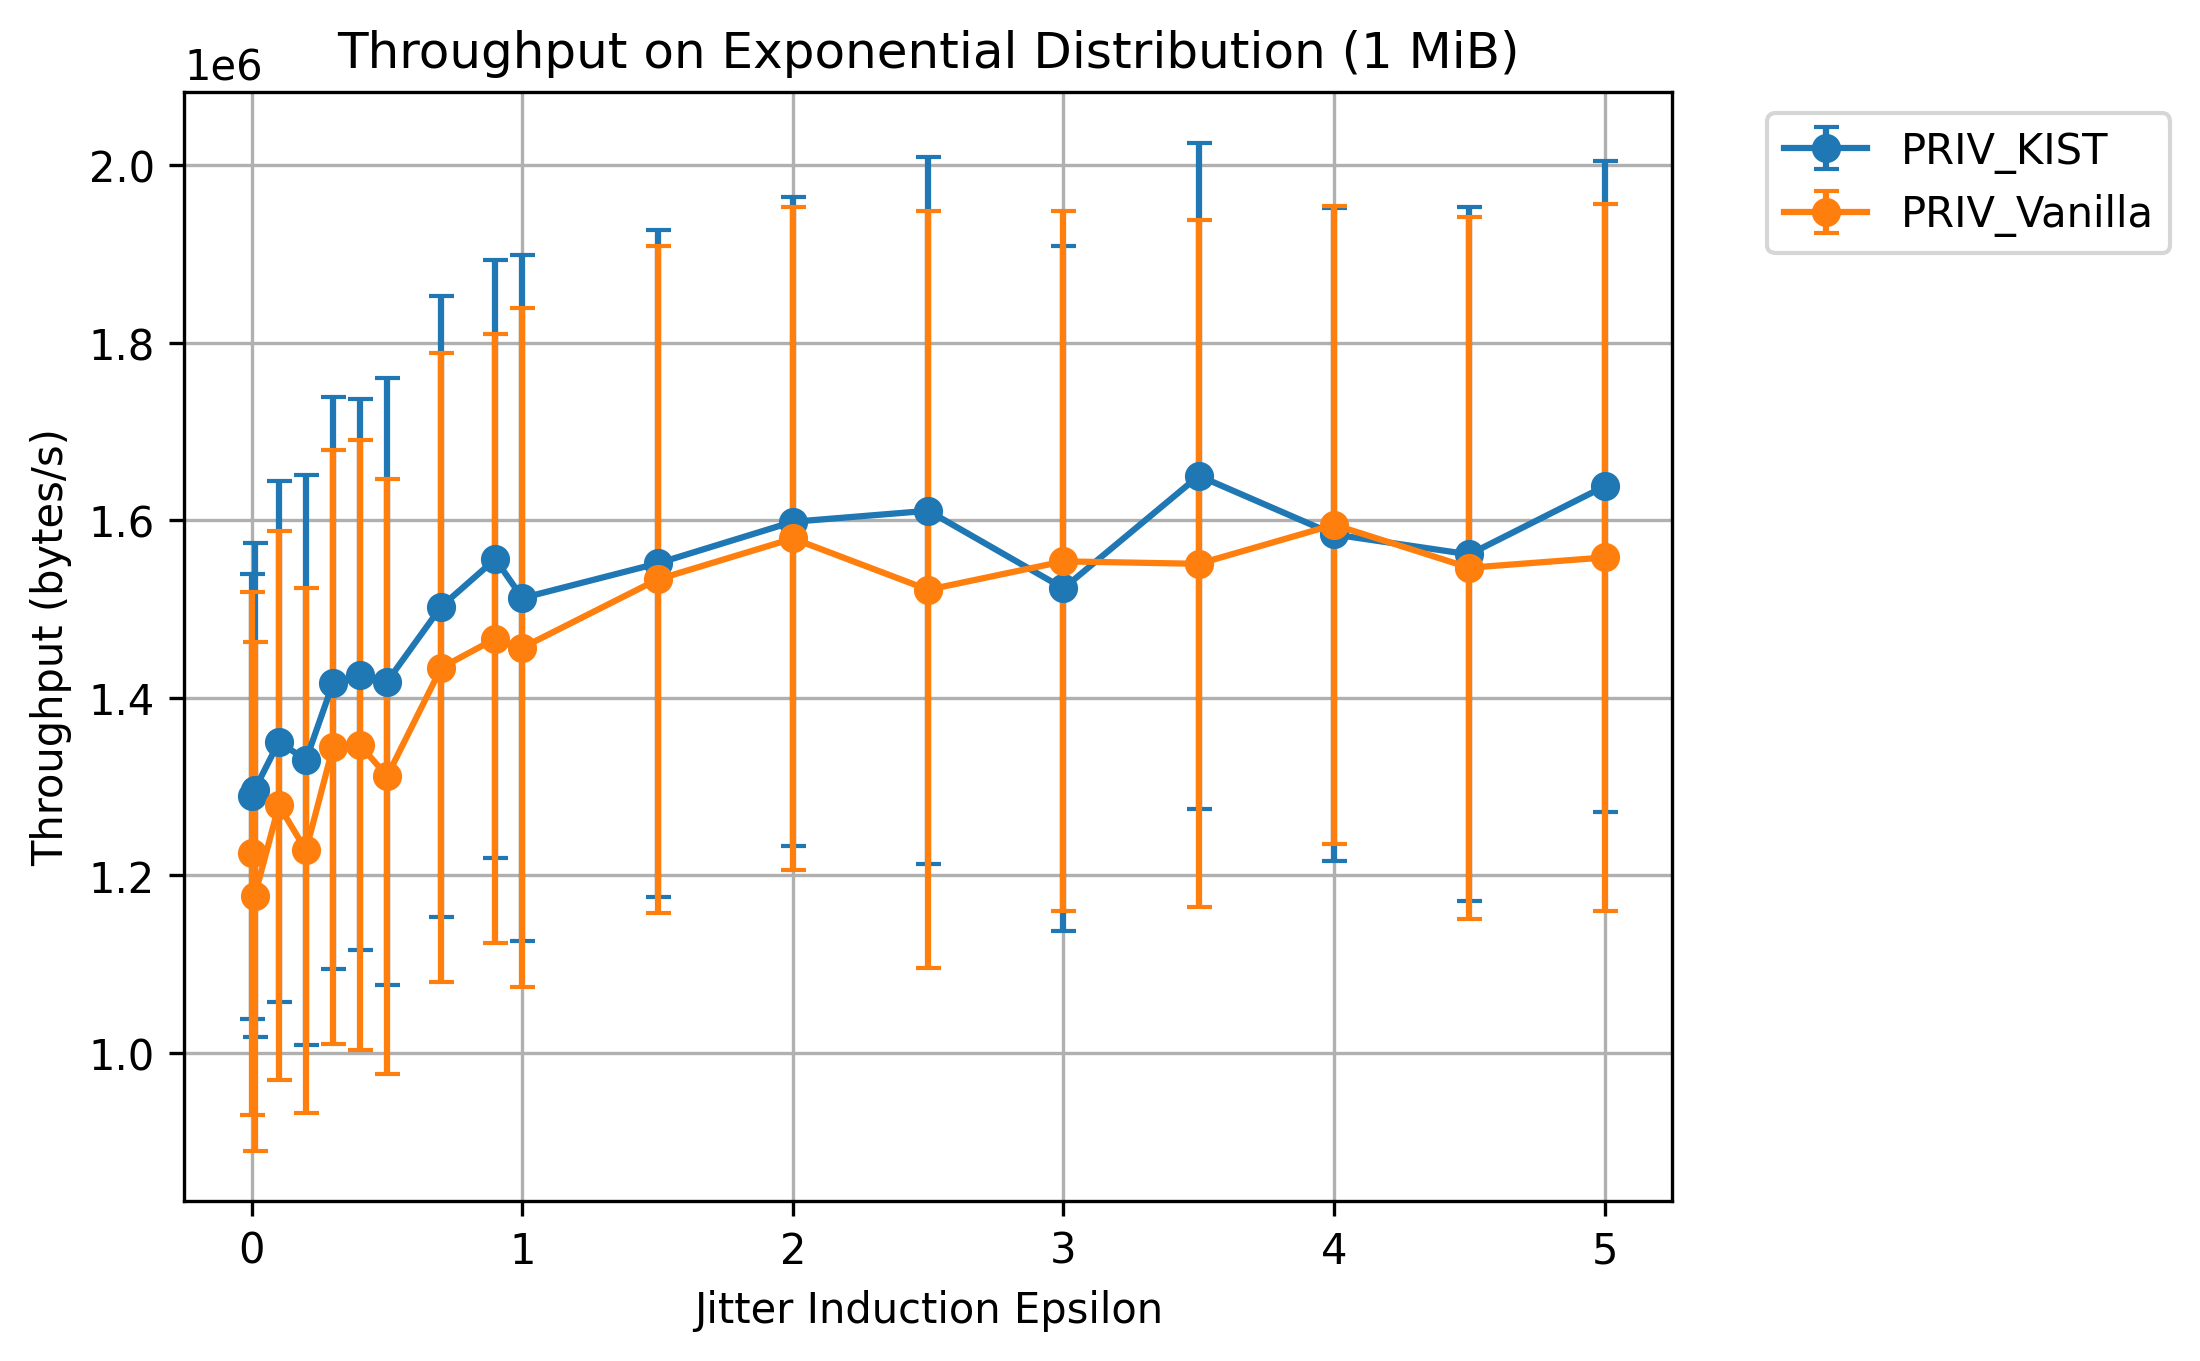
\includegraphics[width=\linewidth]{Chapters/Figures/Plots/Jitter/throughput_jitter_Exponential_1_mib.png}}
    \end{subcaptionbox}
    \hfill
    \begin{subcaptionbox}{Poisson Distribution\label{fig:jitter_throughput_poisson}}[0.45\textwidth]
        {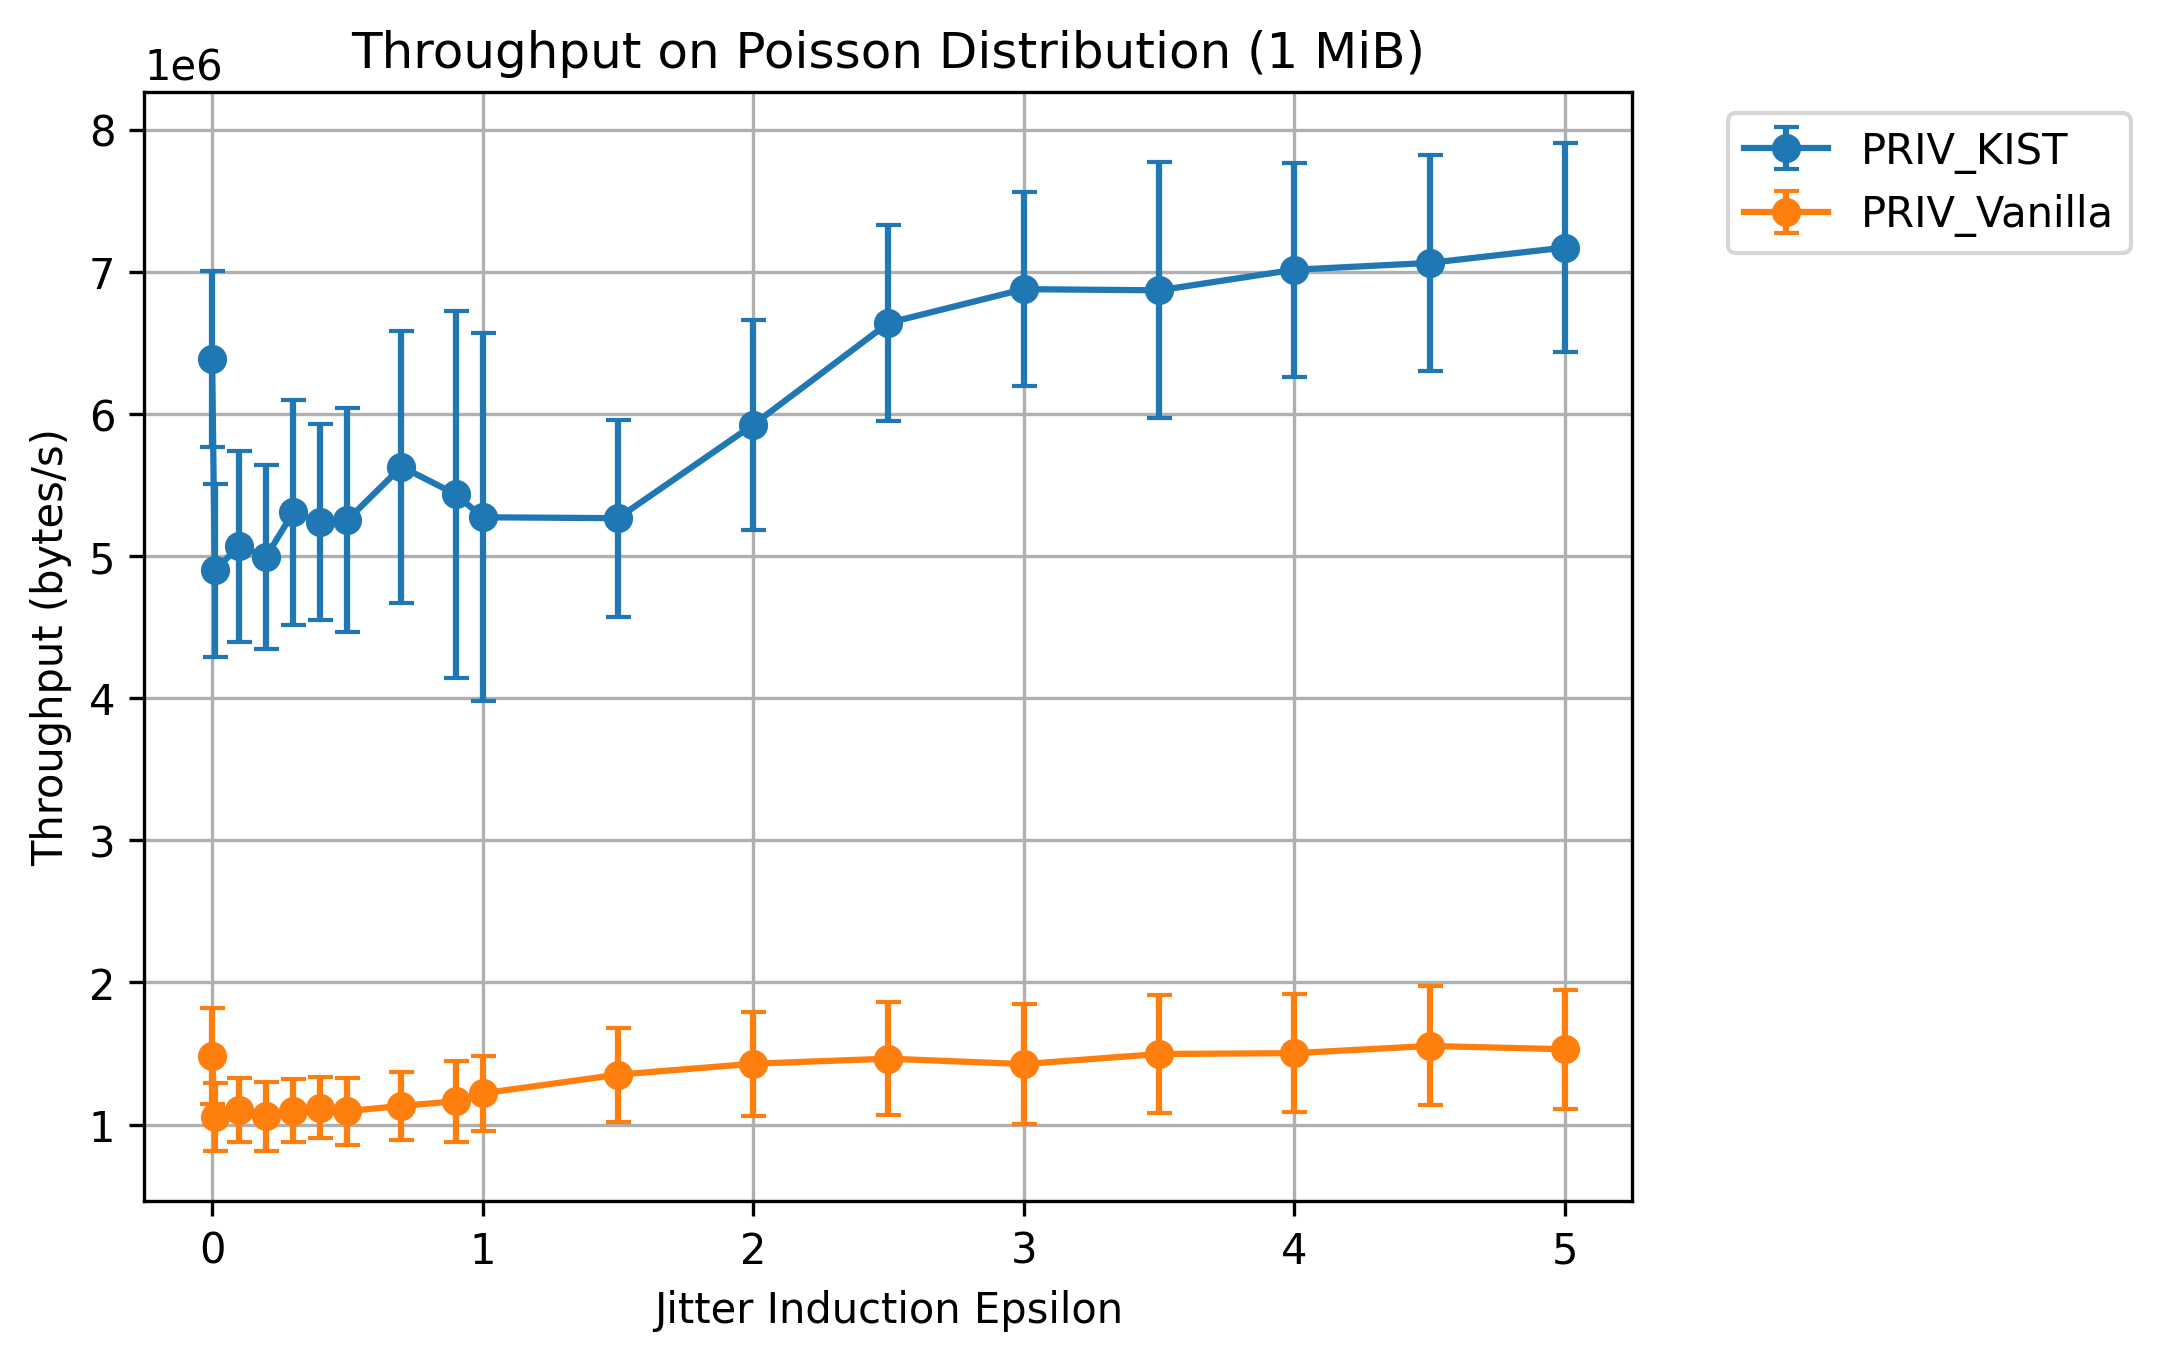
\includegraphics[width=\linewidth]{Chapters/Figures/Plots/Jitter/throughput_jitter_Poisson_1_mib.png}}
    \end{subcaptionbox}
    \hfill
    \begin{subcaptionbox}{All Distributions\label{fig:jitter_throughput_all}}[0.45\textwidth]
        {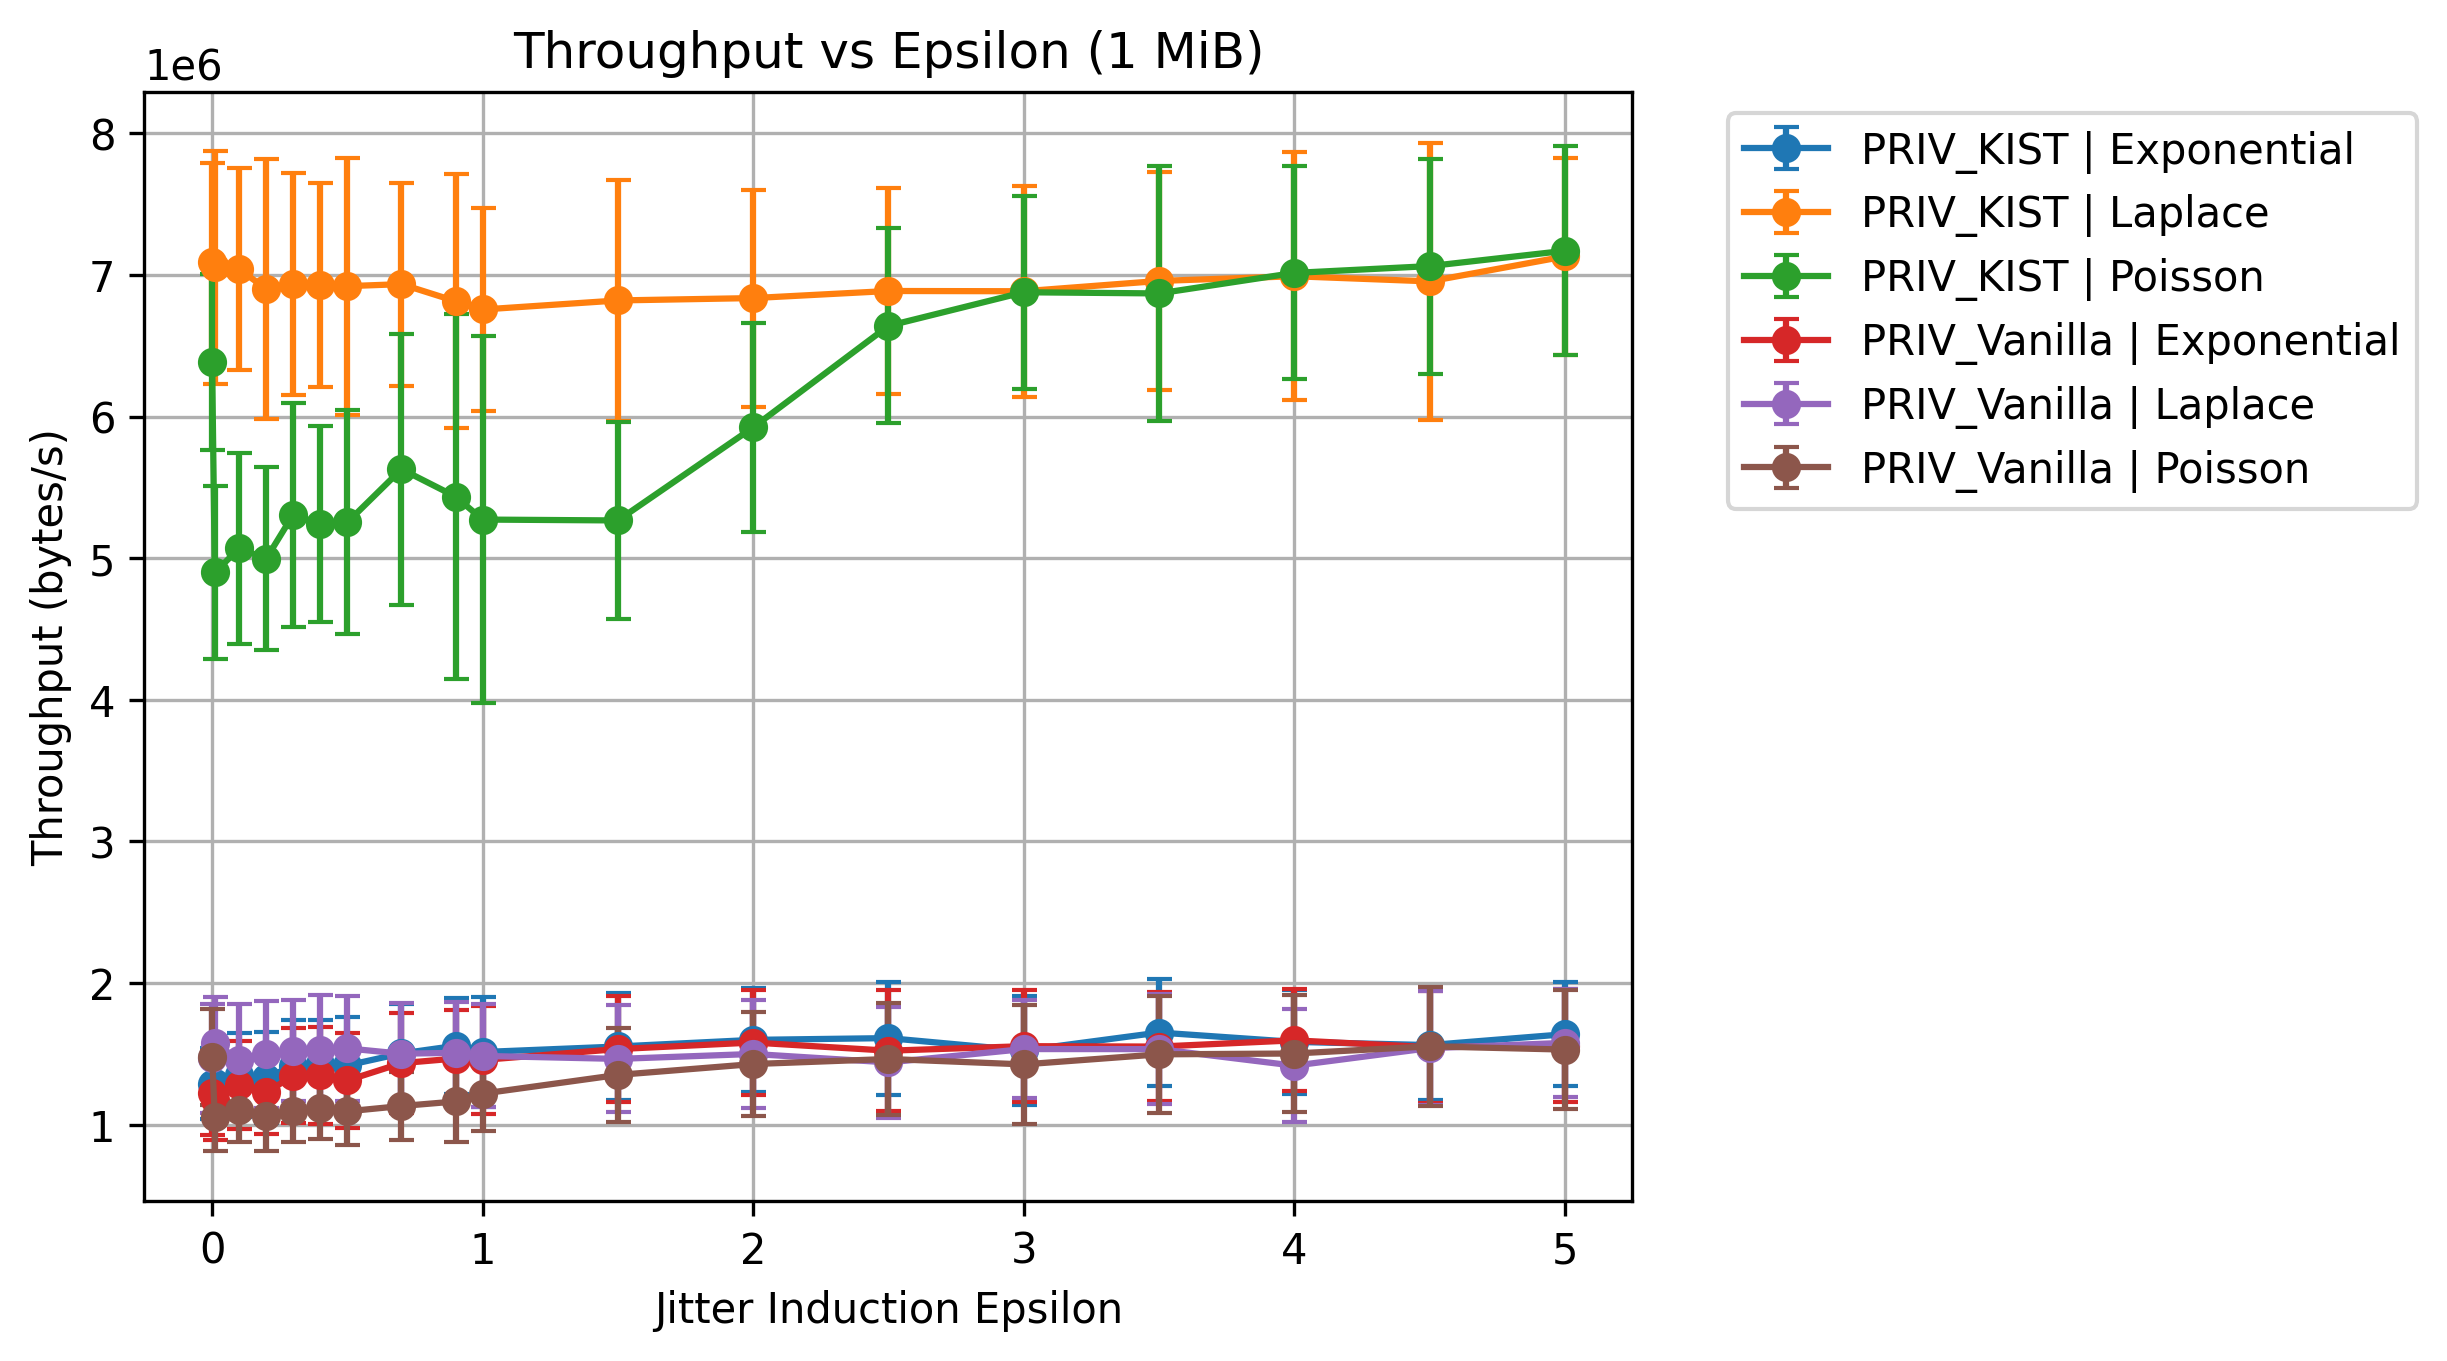
\includegraphics[width=\linewidth]{Chapters/Figures/Plots/Jitter/throughput_jitter_1_mib.png}}
    \end{subcaptionbox}
    \caption{Tor Schedulers and Different Distributions Impact on Throughput}\label{fig:jitter_throughput_analysis}
\end{figure}

Similarly to the latency, the Laplace Distribution shows a stable throughput across all tests, PRIV\_KIST having higher throughput values than PRIV\_Vanilla. The Poisson Distribution shows a decrease in throughput as the $\epsilon$ approaches 0, with a more pronounced decrease for the PRIV\_KIST scheduler, while having higher values than the PRIV\_Vanilla scheduler. The Exponential Distribution also shows a decrease in throughput as the $\epsilon$ approaches 0 for both schedulers and a higher variability in the results. For this distribution, the throughput values are very similar for both schedulers.

In comparison, the Laplace Distribution is the most stable and the PRIV\_KIST scheduler performs better than the PRIV\_Vanilla scheduler. 

\subsubsection{Total Time}\label{sec:performance_evaluation_total_time_jitter_injectors_tor_schedulers}

\begin{figure}[htbp]
    \centering
    \begin{subcaptionbox}{Laplace Distribution\label{fig:jitter_total_time_laplace}}[0.45\textwidth]
        {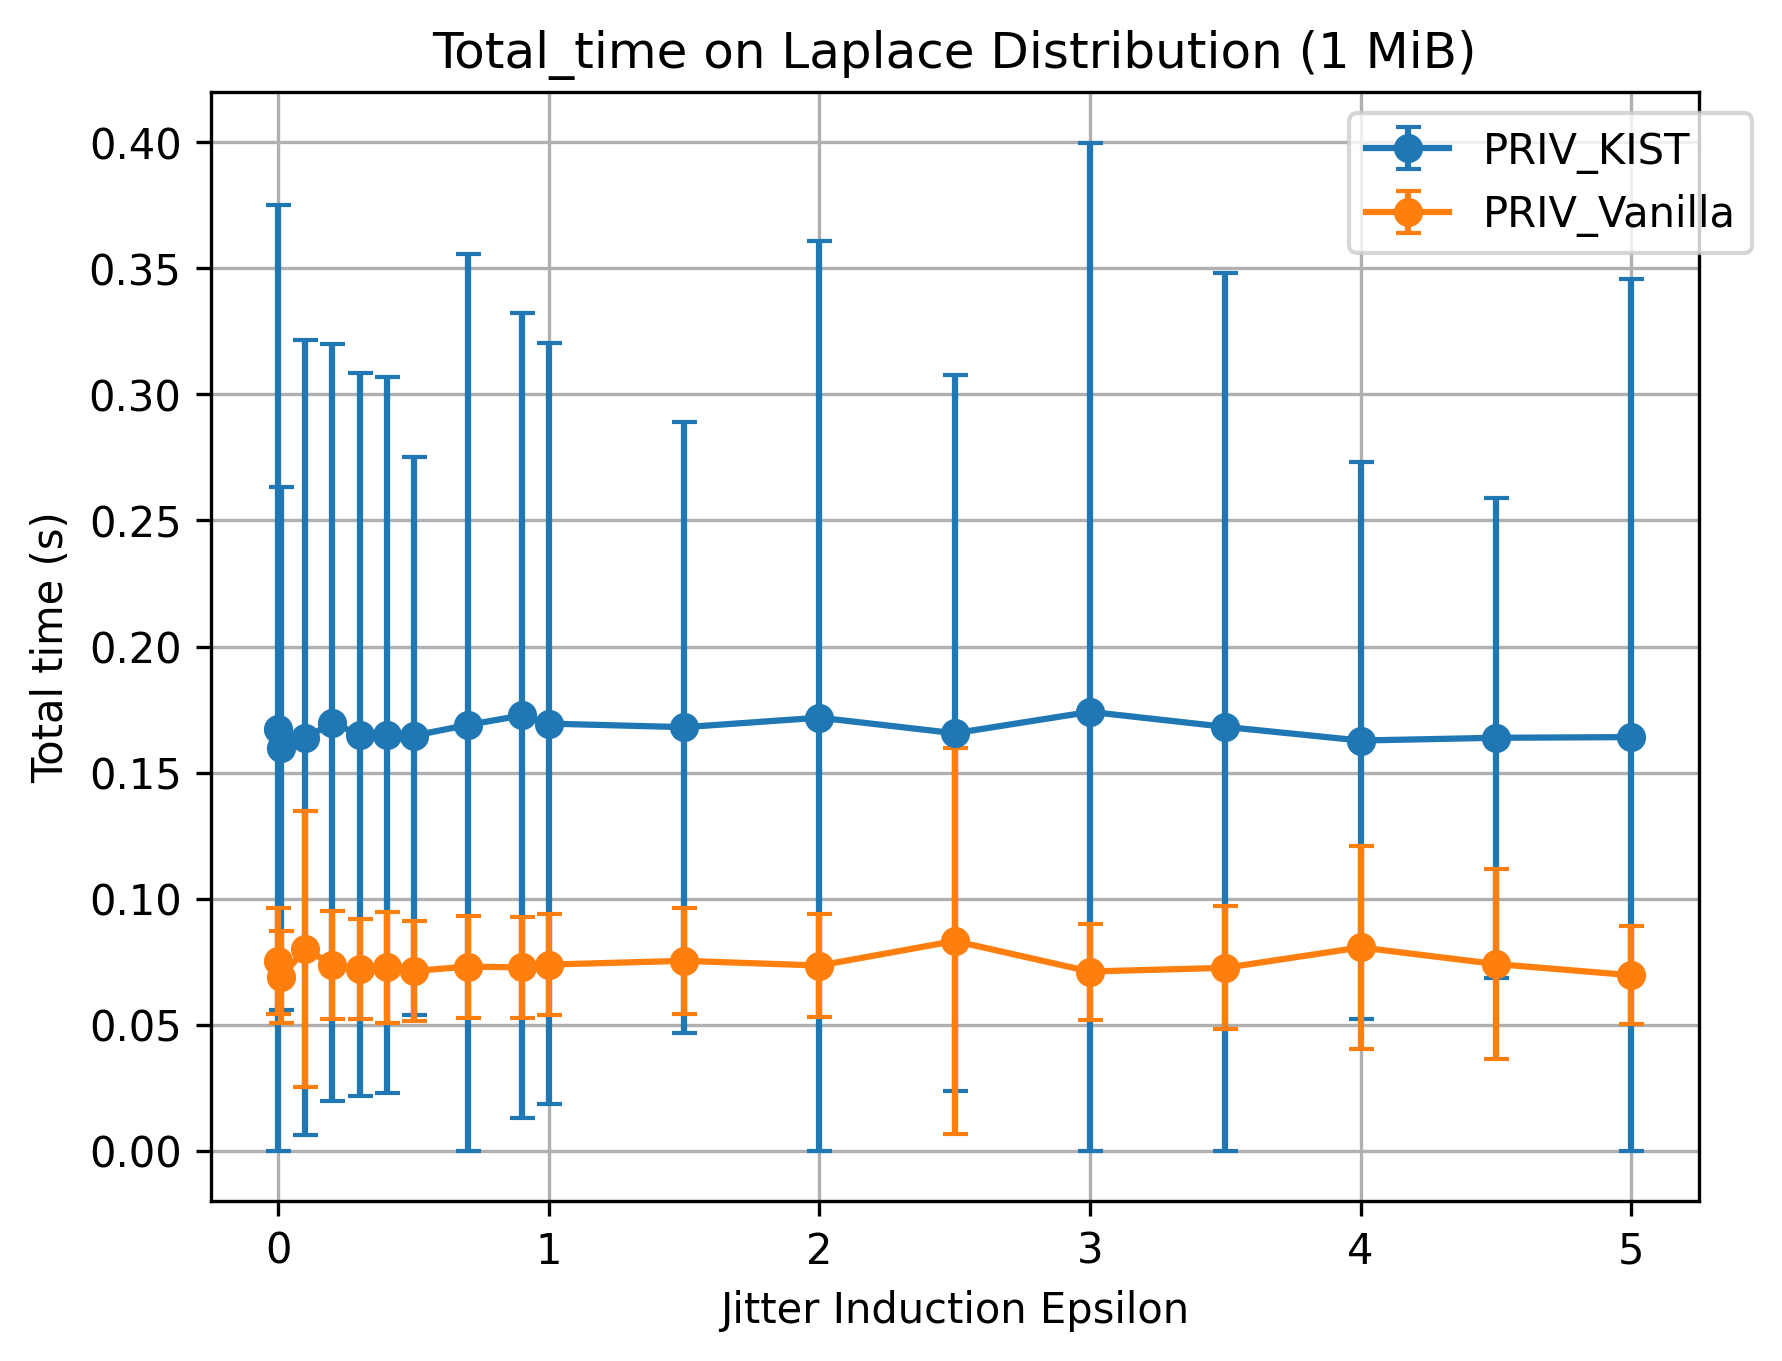
\includegraphics[width=\linewidth]{Chapters/Figures/Plots/Jitter/total_time_jitter_Laplace_1_mib.png}}
    \end{subcaptionbox}
    \hfill
    \begin{subcaptionbox}{Exponential Distribution\label{fig:jitter_total_time_exponential}}[0.45\textwidth]
        {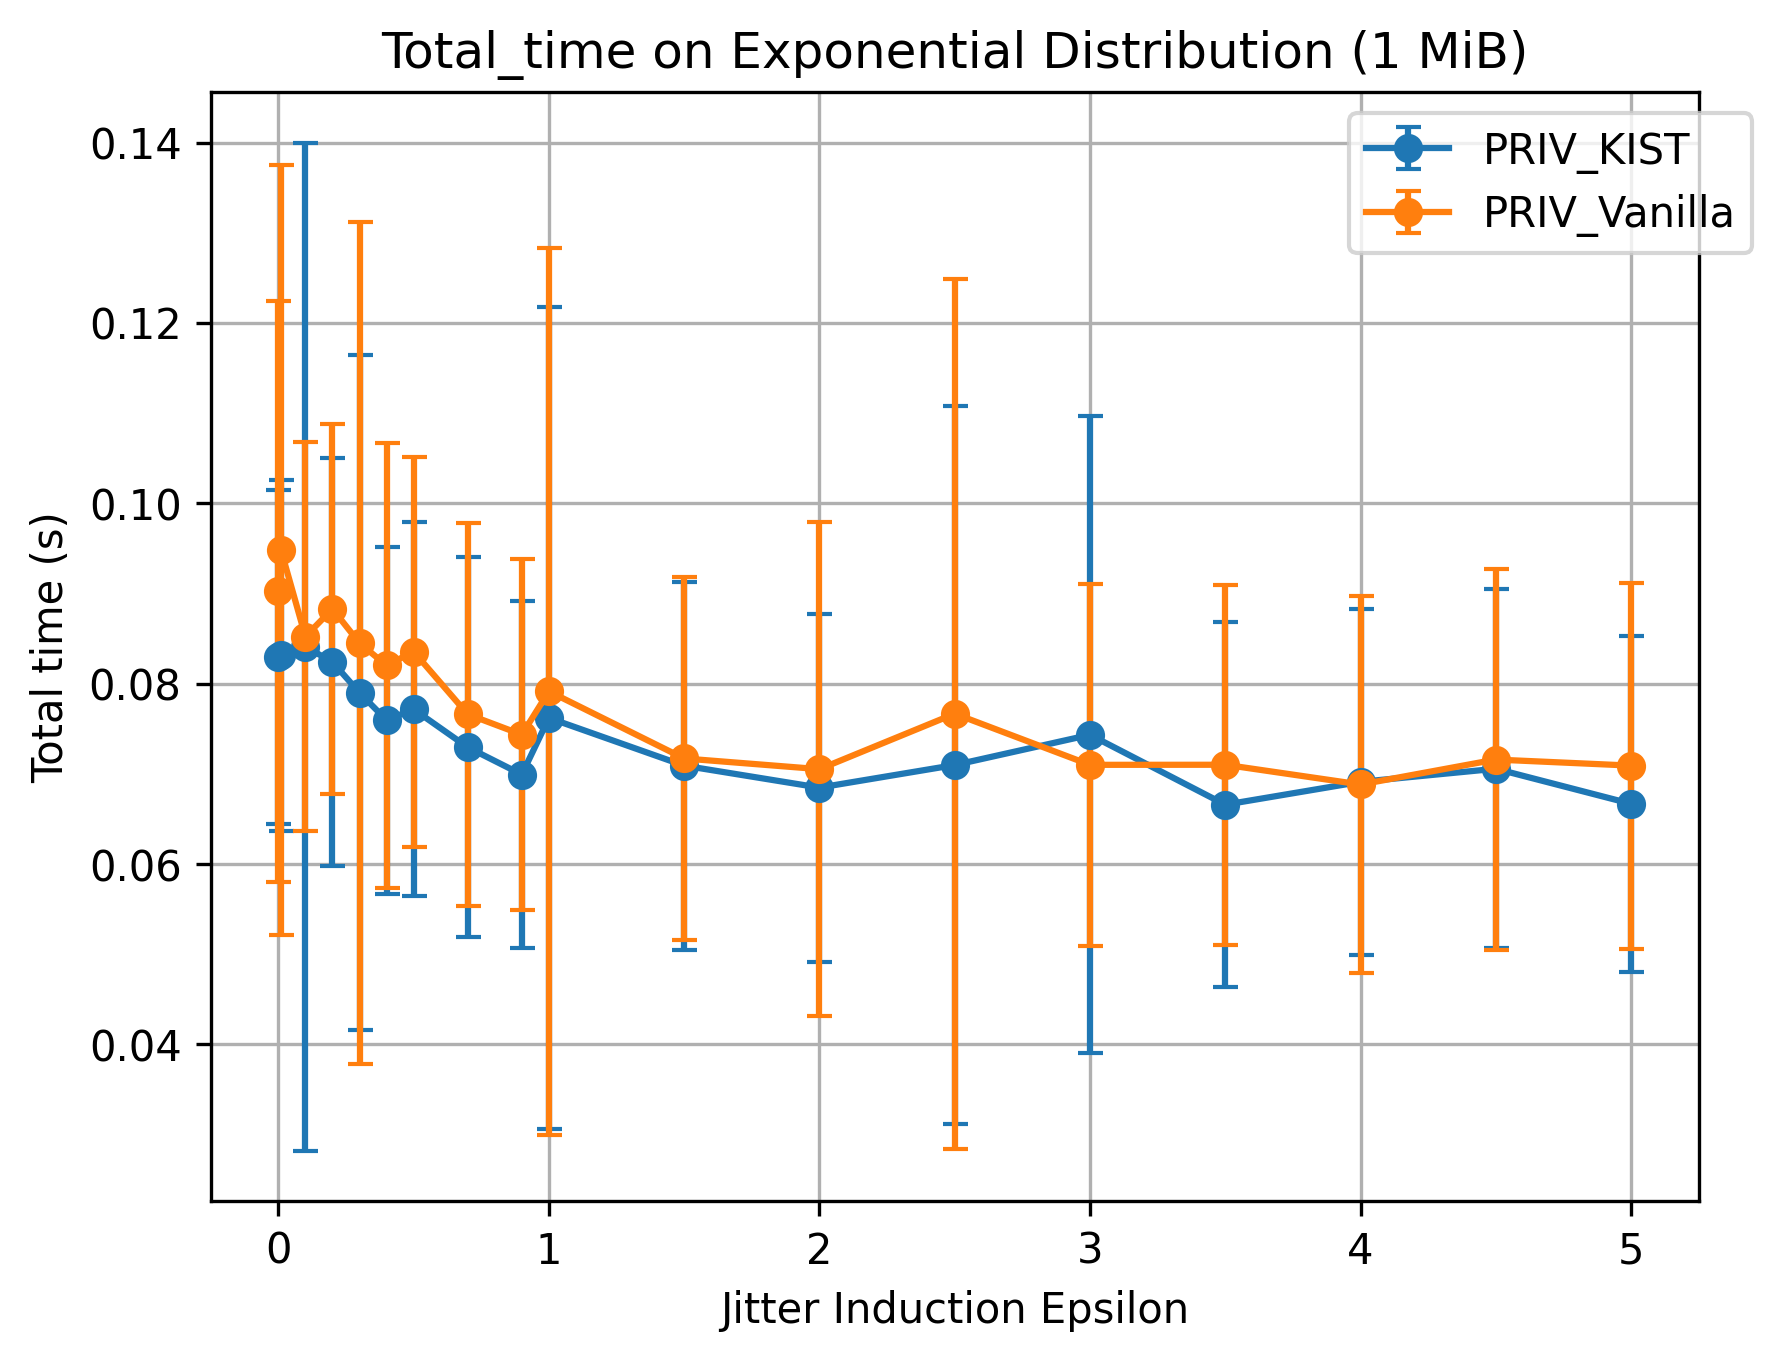
\includegraphics[width=\linewidth]{Chapters/Figures/Plots/Jitter/total_time_jitter_Exponential_1_mib.png}}
    \end{subcaptionbox}
    \hfill
    \begin{subcaptionbox}{Poisson Distribution\label{fig:jitter_total_time_poisson}}[0.45\textwidth]
        {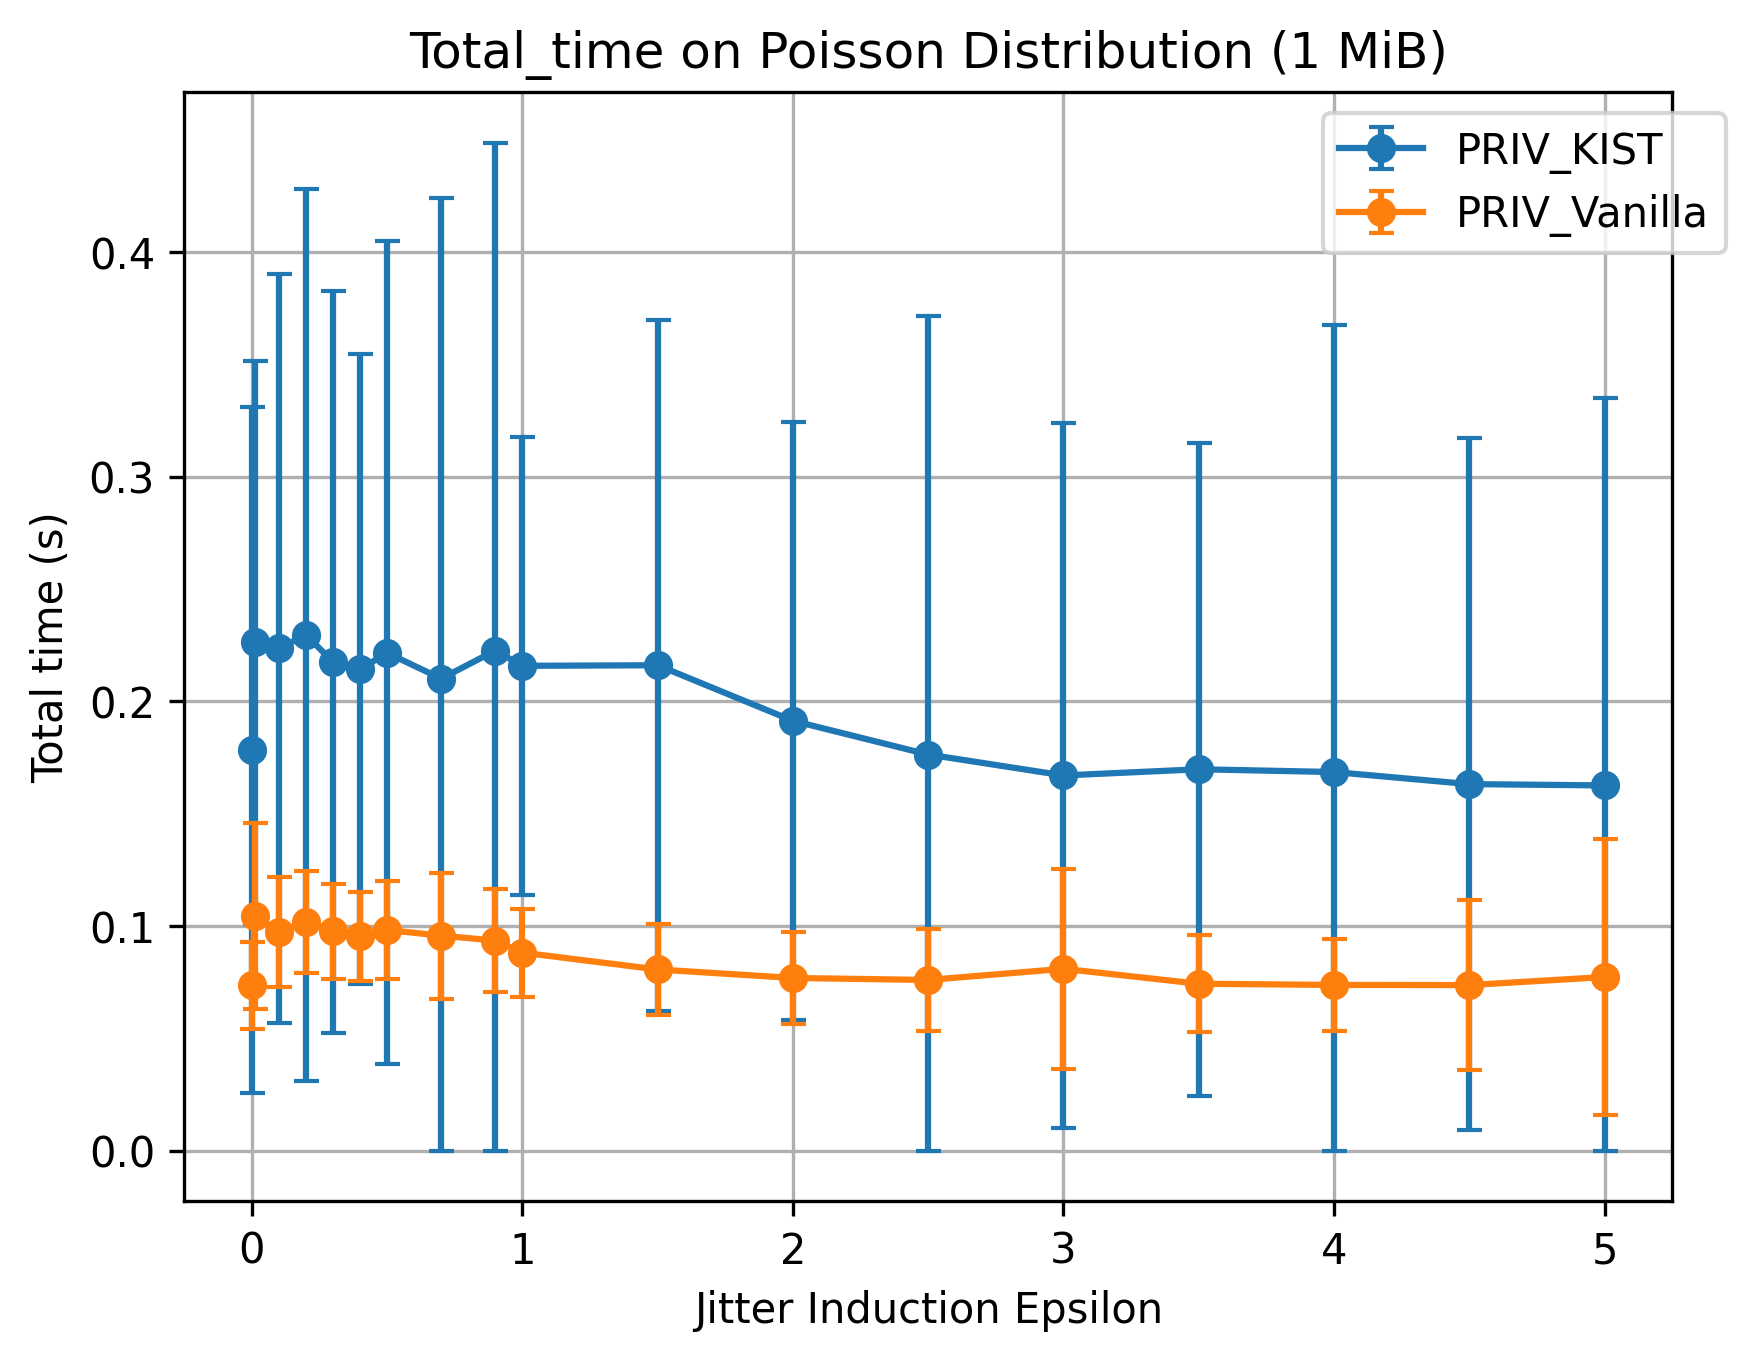
\includegraphics[width=\linewidth]{Chapters/Figures/Plots/Jitter/total_time_jitter_Poisson_1_mib.png}}
    \end{subcaptionbox}
    \hfill
    \begin{subcaptionbox}{All Distributions\label{fig:jitter_total_time_all}}[0.45\textwidth]
        {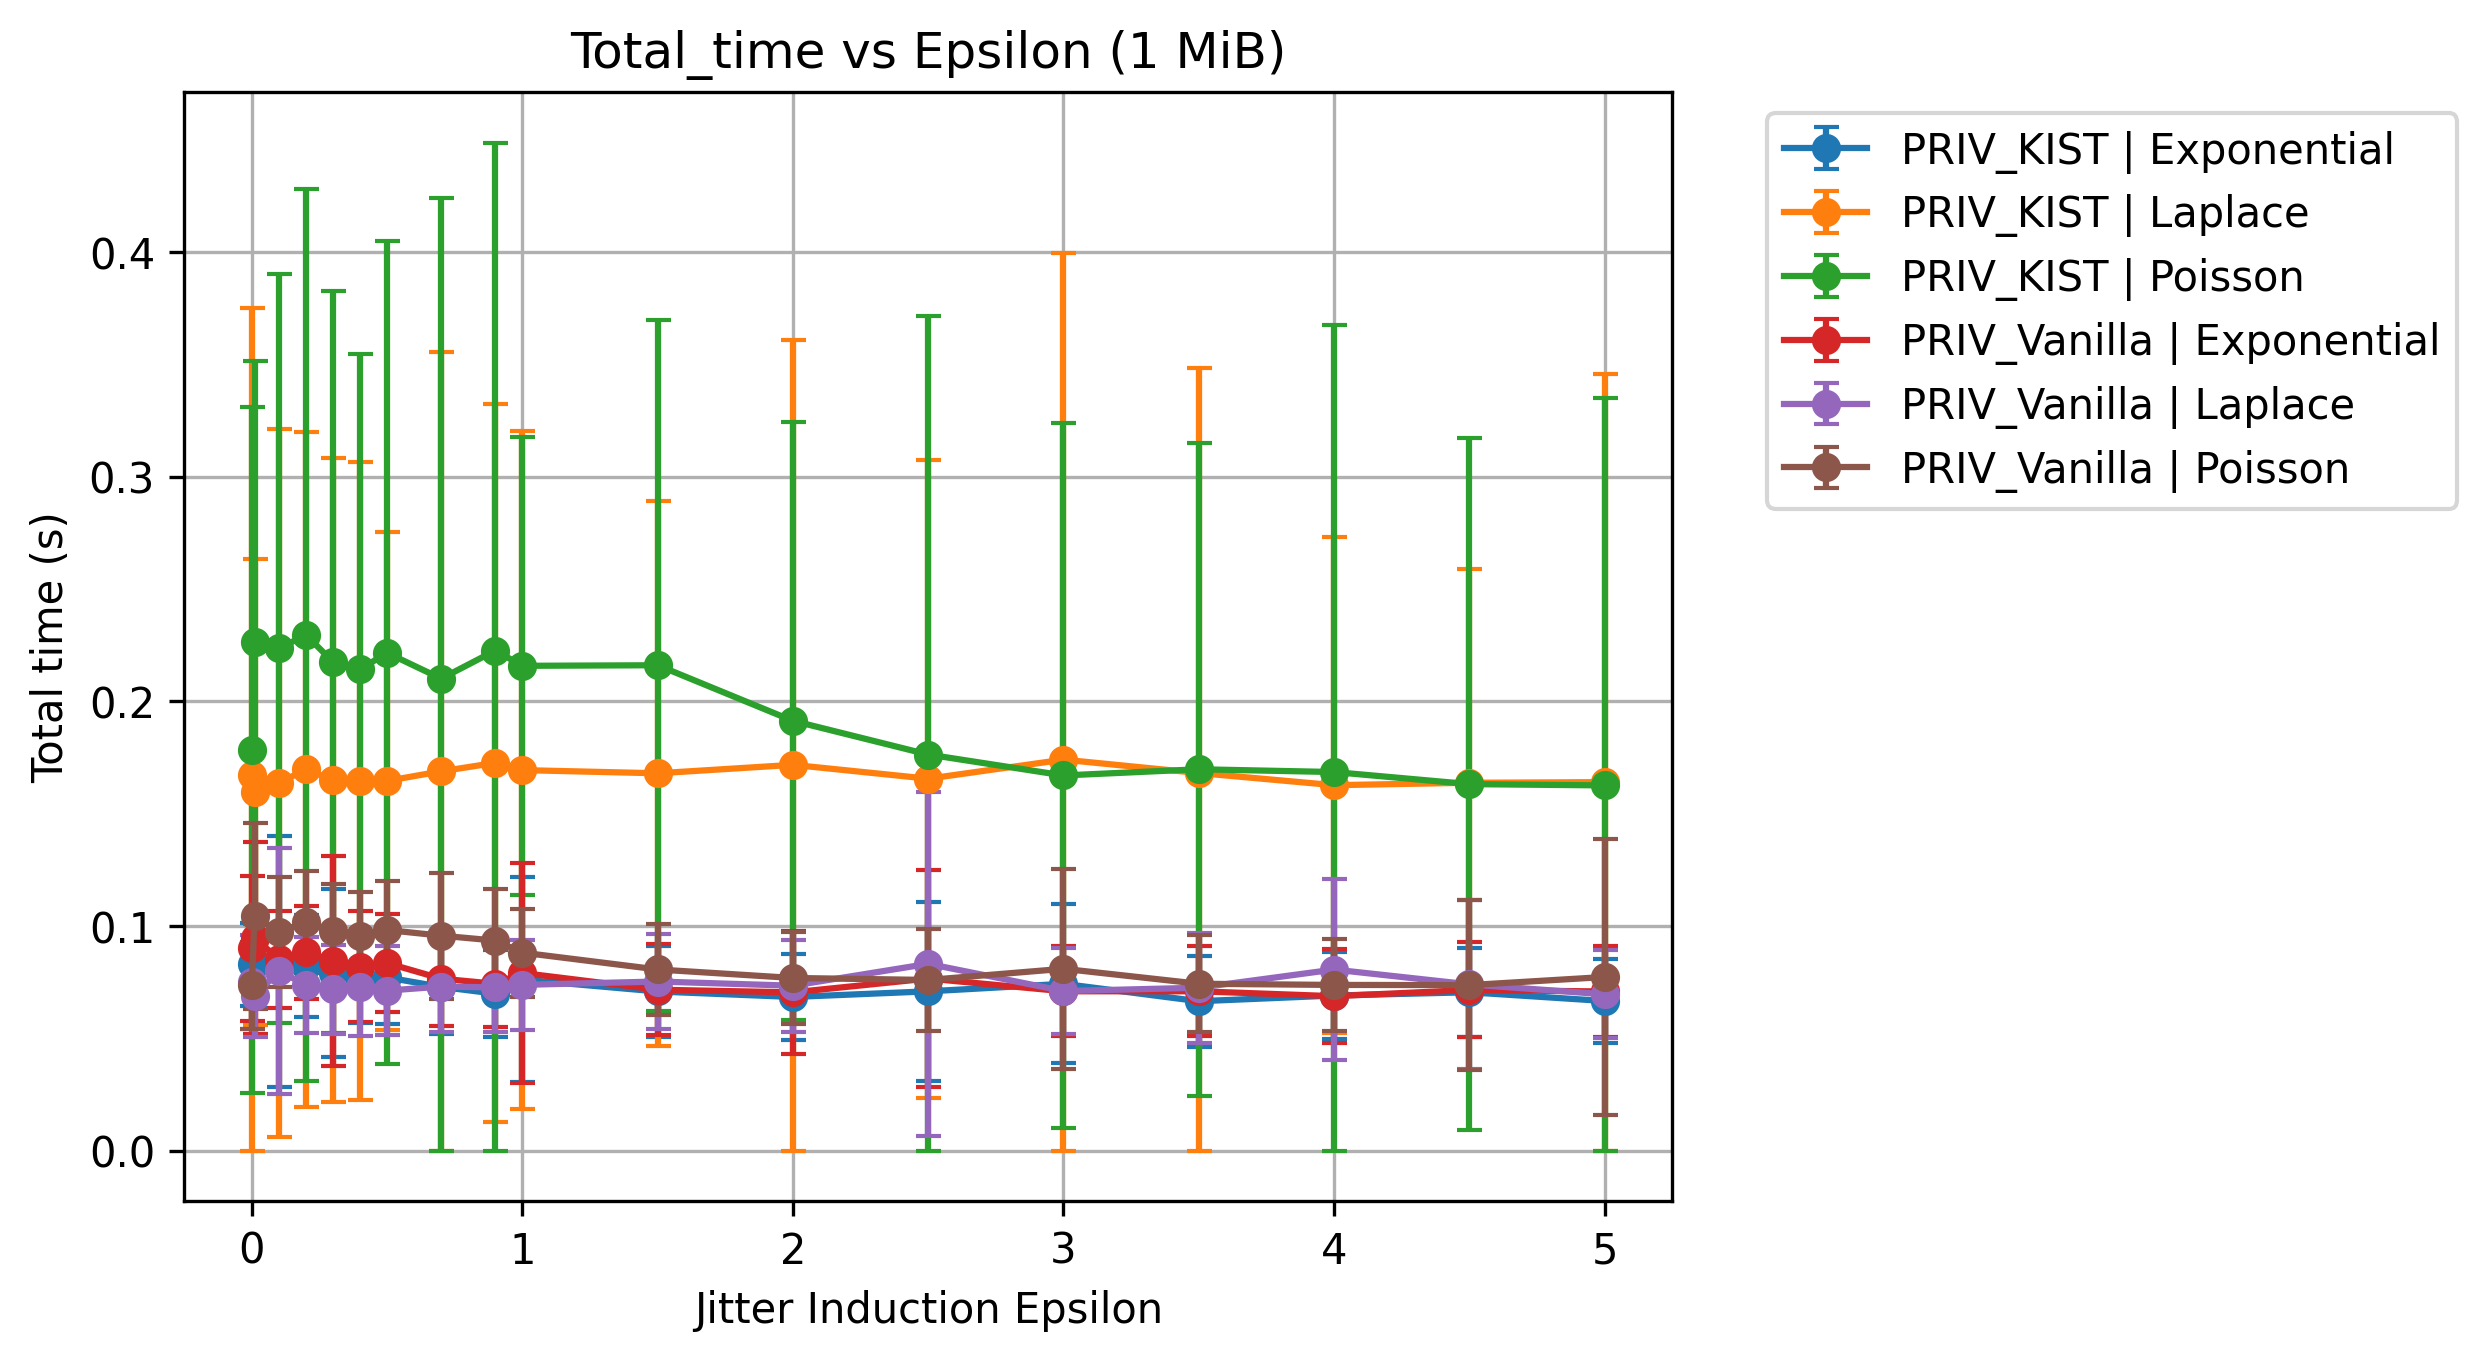
\includegraphics[width=\linewidth]{Chapters/Figures/Plots/Jitter/total_time_jitter_1_mib.png}}
    \end{subcaptionbox}
    \caption{Tor Schedulers and Total Time For Different Distributions}\label{fig:jitter_total_time_analysis}
\end{figure}

The Laplace and Poisson Distributions show a stable total time across all tests, with the PRIV\_Vanilla scheduler having lower total time values than the PRIV\_KIST scheduler. The Exponential Distribution also shows a decrease in total time as the $\epsilon$ increases for both schedulers and a higher variability in the results. For this distribution, the total time values are very similar for both schedulers.

In comparison, all distributions show similar results, in a range of 0.05 to 0.25 seconds, with the Laplace Distribution being the most stable. The PRIV\_Vanilla scheduler performs better than the PRIV\_KIST scheduler for the Laplace and Poisson Distributions, while both schedulers show similar results for the Exponential Distribution. 

\section{Unobservability Evaluation}\label{sec:unobservability_evaluation}

\subsection{Methods and Tools}\label{sec:methods_and_tools}

\subsection{Experimental Observations}\label{sec:experimental_observations_unobservability}

\section{Formal Validation}\label{sec:formal_validation}

\section{Discussion}\label{sec:validation_discussion}

\section{Summary}\label{sec:validation_summary}
